\pdfoutput=1
\PassOptionsToPackage{table}{xcolor}
\documentclass[11pt]{article}

\usepackage[review]{acl}
\usepackage{times}
\usepackage{latexsym}
\usepackage[T1]{fontenc}
\usepackage[utf8]{inputenc}
\usepackage{microtype}
\usepackage{graphicx}
\usepackage{booktabs}
\usepackage{amsmath}
\usepackage{xcolor}
\usepackage{tikz}
\usetikzlibrary{positioning,arrows.meta,calc}
\usepackage{xspace}
\usepackage{url}
\usepackage{enumitem}
\usepackage{array}
\setcounter{dbltopnumber}{1}\renewcommand{\dbltopfraction}{0.75}\renewcommand{\textfraction}{0.07}

\definecolor{ink}{HTML}{0B0B0B}
\definecolor{ink2}{HTML}{52514E}
\definecolor{muted}{HTML}{898781}
\definecolor{axis}{HTML}{C3C2B7}
\definecolor{track}{HTML}{E1E0D9}
\definecolor{heat}{HTML}{5598E7}
\definecolor{barfill}{HTML}{9A9991}
\definecolor{bnews}{HTML}{52514E}
\definecolor{bfinance}{HTML}{52514E}
\definecolor{bscholar}{HTML}{52514E}
\definecolor{blegal}{HTML}{52514E}
\definecolor{brare}{HTML}{52514E}
\definecolor{boxfill}{HTML}{F9F9F7}

\newcommand{\needle}{\textsc{Needle}\xspace}
\newcommand{\ult}{\textit{ceiling}\xspace}
\newcommand{\ndcg}{nDCG@5\xspace}
\newcommand{\hc}[2]{\cellcolor{heat!#1!white}#2}
\newcommand{\shareci}[2]{{\scriptsize\textcolor{ink2}{#1--#2}}}

\title{\needle: A Live Benchmark of Web Search APIs for AI Agents}

\author{Ilya Gusev \quad Matthias Petri \quad Andrey Styskin \\
  Keenable \\
  \texttt{\small\{ilya.gusev,matthias,andrey\}@keenable.ai}}

\begin{document}
\maketitle

\begin{abstract}
AI agents rely on web search APIs, yet no public benchmark tracks how well
these APIs retrieve, and a fixed query set goes stale or gets tuned against.
We present \needle, an open-source benchmark that builds fresh queries and
gold from public sources on every run (one fixed stream excepted), and a
measurement study of the 26 search API configurations it has run. Queries
come hourly from news feeds and daily from seven public registries and
archives. Deterministic matchers or an LLM judge score
each result without annotators, and an engine's score is its share of a
ceiling pooled from all configurations. On the 12 days when all 21 non-variant
engines ran (12.4k query-runs), shares span 15--73\% and paired tests
separate 178 of 210 engine pairs after Bonferroni adjustment. Over 30 days of scholar runs, 23 of 26
configurations find a paper from its title (recall@10 .71--.98) but spread
from .08 to .72 when the query names a detail from its body. Keenable led
all eight weeks, yet on one later day of runs, Perplexity edged past it. Blinded LLM
raters from three vendors agree with one another at $\kappa$ .90--.94 and
with the judge at .77--.79; no human audited the scorers. The evidence
supports choosing a search API by bench and by pairwise tests, not by rank.
Code, data and dashboard are public; links are withheld for review.
\end{abstract}

\section{Introduction}

An agent that searches for a detail from the body of a recent paper, such as
the phrase ``gap rent regularity'', can read the paper only if its search
API returns it. From 29 September to 28 October 2026, Keenable put
the paper in its top ten for 72\% of such body-keyword queries and ChatGPT
search
for 8\%. Yet both found papers from their titles more than 80\% of the
time (Figure~\ref{fig:results}a). Public evidence for choosing between such
APIs is thin. IR test collections target document rankers over fixed
corpora, and their labels age (``Fed rate decision'' changes every six
weeks). Agent benchmarks such as BrowseComp score the whole agent, so a weak
retriever hides behind a strong model.

\needle measures the search API alone, on five benches
(Figure~\ref{fig:pipeline}). Its unit
of evaluation is one search request (retried on errors): a query in, up to
$k$ results out, scored on
the title, URL and snippet the agent would see. Every run generates fresh
queries and gold from public sources, so no fixed test set accumulates (the
rare bench and registry facts excepted; Limitations). Where the gold has a canonical
identity, such as an arXiv id, a reporter citation or a 10-Q figure, a
deterministic matcher checks the results. Where relevance is graded, as for
news, an LLM judge rates each result. Each engine's score is a share of a
ceiling pooled from all configurations. Scores rest on snippets and, for two
benches, on one judge; we audit both with LLMs, not humans (Limitations).
We contribute:
\begin{itemize}[nosep,leftmargin=1.2em]
\item A benchmark that regenerates queries and gold on every run and scores
  them without annotators. On its two judged benches, blinded LLM raters
  from three vendors agree with the judge at $\kappa$ .77--.79 on 1,200
  results (\S\ref{sec:results}, Appendix~\ref{app:checks}).
\item A normalization by a pooled ceiling that no single engine drives:
  scoring each engine against a ceiling pooled without it moves its overall
  share by at most 0.8 points (\S\ref{sec:results}).
\item Public results for 26 configurations: over 12 days, overall shares
  span 15--73\% (Table~\ref{tab:results}), and body-keyword queries
  separate engines that title queries do not (Figure~\ref{fig:results}).
\end{itemize}
The combination is new; each scoring ingredient follows prior work
(\S\ref{sec:related}).

\begin{figure*}[t]
\centering
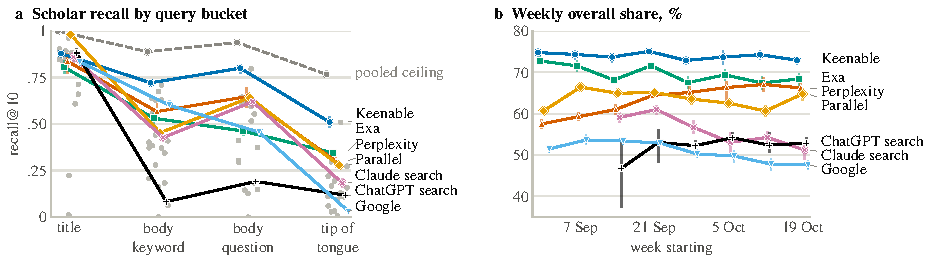
\includegraphics[width=\textwidth]{fig_results.pdf}
\caption{Most engines find a paper from its title but spread apart when the
query names a detail from its body (a), and Keenable leads every week
while the ranks below it shift (b). (a) Scholar recall@10 per query bucket,
31 runs from 29 September to 28 October 2026, 2,600--3,005 query-runs per line and bucket;
lines: the seven engines of (b); grey dots: the other 19 configurations;
dashed: the pooled ceiling. (b) Overall share per ISO week, 31 August to
25 October 2026; ChatGPT and Claude search start on 14 September;
the pool grew from 18 to 25 configurations.
Points: query-weighted means; vertical lines: 95\% run-level bootstrap
intervals. Scores and failures as the dashboard publishes them
(Table~\ref{tab:results}).}
\label{fig:results}
\end{figure*}

\begin{figure*}[t]
\centering
\scriptsize
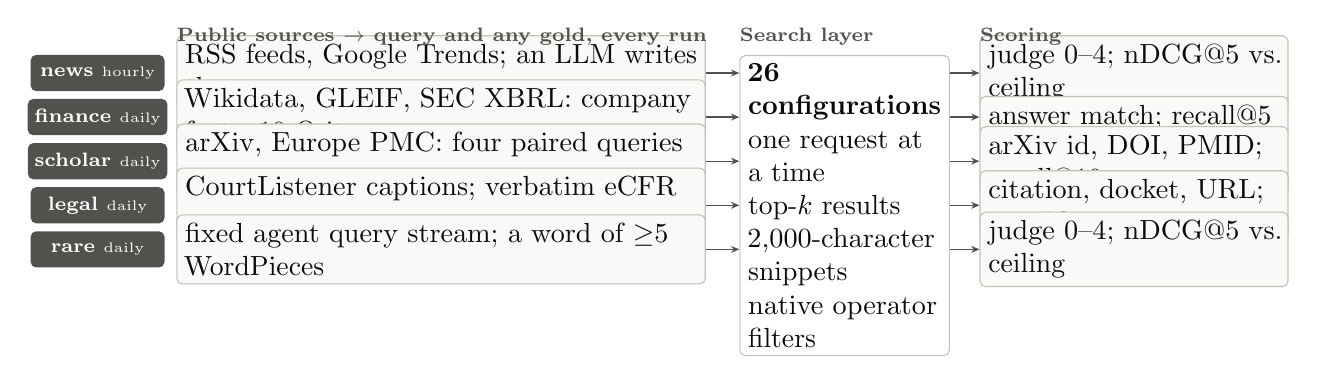
\begin{tikzpicture}[
  x=1cm, y=1cm,
  box/.style={draw=axis, fill=boxfill, rounded corners=2pt, inner sep=3pt, align=left, text=ink, execute at begin node={\hyphenpenalty10000\relax}},
  tag/.style={rounded corners=2pt, inner sep=2.5pt, text=white, font=\scriptsize\bfseries, align=center},
  head/.style={text=ink2, font=\scriptsize\bfseries, anchor=south west, inner sep=0pt},
  flow/.style={-{Stealth[length=3pt,width=2.5pt]}, ink2, line width=0.5pt},
]
\def\rowh{0.56}
\def\boxh{0.46}
\pgfmathsetmacro{\tallh}{4*\rowh+\boxh}
\foreach \i/\name/\col/\cad/\gen/\score in {
  0/news/bnews/hourly/{RSS feeds, Google Trends; an LLM writes the query}/{judge 0--4; \ndcg vs.\ ceiling},
  1/finance/bfinance/daily/{Wikidata, GLEIF, SEC XBRL: company facts, 10-Q items}/{answer match; recall@5},
  2/scholar/bscholar/daily/{arXiv, Europe PMC: four paired queries per paper}/{arXiv id, DOI, PMID; recall@10},
  3/legal/blegal/daily/{CourtListener captions; verbatim eCFR spans}/{citation, docket, URL; recall@5},
  4/rare/brare/daily/{fixed agent query stream; a word of $\geq$5 WordPieces}/{judge 0--4; \ndcg vs.\ ceiling}%
}{
  \pgfmathsetmacro{\yy}{-\i*\rowh}
  \node[tag, fill=\col, minimum width=1.7cm, minimum height=\boxh cm] (T\i) at (0.85,\yy) {\name~{\mdseries\tiny\cad}};
  \node[box, text width=6.5cm, minimum height=\boxh cm, anchor=west] (B\i) at (1.85,\yy) {\gen};
  \node[box, text width=3.7cm, minimum height=\boxh cm, anchor=west] (D\i) at (12.05,\yy) {\score};
}
\node[box, text width=2.45cm, minimum height=\tallh cm, anchor=north west, fill=white] (C) at (9.0,{\boxh/2}) {\textbf{26 configurations}\\one request at a time\\top-$k$ results\\2,000-character snippets\\native operator filters};
\foreach \i in {0,...,4}{
  \draw[flow] (B\i.east) -- (B\i.east -| C.west);
  \draw[flow] (D\i.west -| C.east) -- (D\i.west);
}
\node[head] at (1.85,{\boxh/2+0.12}) {Public sources $\rightarrow$ query and any gold, every run};
\node[head] at (9.0,{\boxh/2+0.12}) {Search layer};
\node[head] at (12.05,{\boxh/2+0.12}) {Scoring};
\end{tikzpicture}
\caption{Every run draws its queries, and any gold, from public sources. One
search layer sends each query, without its gold, to every configuration; the
scorer checks the returned title, URL and snippet against the gold, or
the judge rates them.}
\label{fig:pipeline}
\end{figure*}

\section{The Benchmark}
\label{sec:bench}

Figure~\ref{fig:pipeline} shows the five benches. A \emph{configuration} is
one search API at one setting: we test 26, from 20 vendors, five of them
variants such as a vendor's fast or realtime mode. We call a configuration
under evaluation an \emph{engine}. A query issued in one run is a
\emph{query-run}.

\begin{table*}[t]
\centering\footnotesize
\setlength{\tabcolsep}{3pt}
\renewcommand{\arraystretch}{0.8}
\begin{tabular}{@{}lrlrrrrrrr@{}}
\toprule
Engine & \multicolumn{2}{c}{Overall share, \%} & Scholar & News & Finance & Rare & Legal & Failed, \% & Latency \\
\cmidrule(lr){2-3}
 & mean & 95\% CI & R@10 & \ndcg & R@5 & \ndcg & R@5 & requests & $p_{50}$, ms \\
\midrule
\textit{ceiling (pooled)} & \textit{100} & & \textit{.901} & \textit{1} & \textit{.993} & \textit{1} & \textit{.971} & & \\
Keenable & 73.2 & \shareci{72.3}{74.1} & \textbf{.731} & .609 & .903 & \textbf{.508} & \textbf{.797} & 0.0 & 135 \\
Exa & 68.5 & \shareci{67.4}{69.4} & .563 & .599 & \textbf{.922} & .476 & .771 & 0.3 & 2,132 \\
Perplexity & 66.9 & \shareci{65.3}{68.5} & .578 & .640 & .895 & .468 & .674 & 0.0 & 433 \\
Parallel & 64.9 & \shareci{63.6}{66.1} & .587 & .535 & .907 & .387 & .734 & 0.8 & 2,660 \\
Brave (LLM ctx) & 64.6 & \shareci{63.4}{65.6} & .533 & \textbf{.642} & .858 & .454 & .658 & 0.0 & 1,112 \\
Linkup & 57.6 & \shareci{56.1}{58.9} & .470 & .567 & .797 & .400 & .570 & 0.0 & 1,212 \\
Brave & 57.3 & \shareci{56.2}{58.4} & .488 & .557 & .769 & .354 & .621 & 0.0 & 487 \\
Context & 57.1 & \shareci{55.4}{58.6} & .598 & .469 & .782 & .339 & .576 & 0.0 & 866 \\
DeepSeek & 56.9 & \shareci{55.8}{57.9} & .271 & .635 & .818 & .387 & .676 & 0.0 & 551 \\
You.com & 55.8 & \shareci{54.7}{56.9} & .471 & .553 & .747 & .343 & .602 & 0.0 & 486 \\
ChatGPT search\smash{$^{\dagger\S}$} & 51.5 & \shareci{49.4}{53.1} & .300 & .340 & .809 & .366 & .697 & 11.1 & 43,831 \\
Kagi\smash{$^\S$} & 51.3 & \shareci{49.9}{52.6} & .560 & .301 & .728 & .275 & .617 & 7.6 & 1,275 \\
Firecrawl & 50.7 & \shareci{49.2}{52.0} & .488 & .286 & .820 & .265 & .598 & 0.0 & 688 \\
Octen & 50.2 & \shareci{48.8}{51.7} & .307 & .511 & .730 & .322 & .586 & 0.0 & 197 \\
Google (Serper) & 47.7 & \shareci{46.8}{48.6} & .475 & .262 & .738 & .255 & .582 & 0.0 & 1,785 \\
Claude search\smash{$^{\dagger\S}$} & 45.1 & \shareci{42.7}{47.6} & .498 & .276 & .685 & .195 & .525 & 35.9 & 33,906 \\
TinyFish\smash{$^\S$} & 44.5 & \shareci{43.0}{45.9} & .429 & .256 & .730 & .220 & .521 & 29.0 & 1,904 \\
Bing (SearchAPI) & 44.1 & \shareci{41.1}{46.8} & .416 & .288 & .675 & .173 & .586 & 0.4 & 2,008 \\
Jina & 43.8 & \shareci{42.4}{45.1} & .492 & .210 & .726 & .163 & .523 & 4.9 & 17,272 \\
Tavily & 42.6 & \shareci{41.5}{43.7} & .303 & .303 & .828 & .284 & .361 & 0.1 & 1,999 \\
Ceramic & 14.7 & \shareci{13.9}{15.7} & .001 & .040 & .441 & .109 & .137 & 0.1 & 99 \\

\bottomrule
\end{tabular}
\caption{Overall shares of the ceiling span 15--73\%; paired tests separate
188 of the 210 engine pairs, 178 after a Bonferroni adjustment and 164 under
two further checks (\S\ref{sec:results}). Data: the dashboard's 276 runs, 17--28
October 2026, in which all 21 listed engines ran (12.4k query-runs;
Table~\ref{tab:accounting}); the ceiling also pools the variants
that ran beside them.
$^\dagger$A model's server-side search tool; latency includes answer
generation. $^\S$Rank depends on excluded account-side failures: scoring
them zero or at the ceiling puts Claude search at 34.7--52.0, TinyFish at
37.6--52.0, Kagi at 47.5--53.2 and ChatGPT search at 48.2--54.5
(Appendix~\ref{app:checks}). Bench
cells: absolute metric, best in bold; italic: the ceiling. Failed: all failed
requests, account-side ones included. Intervals: 95\%
run-level bootstraps (sampling uncertainty, not scorer error). Latency:
per-run median on news.}
\label{tab:results}
\end{table*}

\subsection{Query generation}

\textbf{News.} Each hour an LLM writes a terse query on the specific event
of the newest item from each of 124 feeds and of the Google Trends RSS for
52 US geographies, and refuses evergreen items. Each run samples 20
queries round-robin over topics. \textbf{Finance.} Queries ask for
registry facts such as a CEO or a ticker (Wikidata, GLEIF), quarterly 10-Q
line items (SEC XBRL) or a filing by description. \textbf{Scholar.} Each paper yields a \emph{title} query with
case and punctuation stripped; a \emph{body keyword} query on a detail
absent from title and abstract; a \emph{body question} that asks for the
same fact in prose; and a \emph{tip-of-tongue} description with every name
and exact value banned. A paper enters only if all four queries pass, so the
buckets are paired. \textbf{Legal.} Recent opinions from 14 federal courts
yield one caption-style query each; the gold is the citation, docket number
and CourtListener id. Sections of the Code of Federal Regulations (CFR)
yield an LLM query built on one verbatim span of two to eight words, quoted
in one variant in four; a query that leaks the citation is rejected
(Appendix~\ref{app:leak}). \textbf{Rare.} English agent queries from a
public stream that contain a word WordPiece splits into five or more pieces.
\textbf{Operators.} Agent queries often carry operators
\citep{meng2026textranking,pezzuti2026agentssearch}, so at least half of
the legal queries and of the finance money and filing queries carry a quoted
phrase, \texttt{site:}, \texttt{after:} or \texttt{before:}. The search
layer maps each operator to the engine's native filter where one exists
(Appendix~\ref{app:ops}).

\subsection{Scoring}
\label{sec:scoring}

\textbf{Graded relevance with a pooled ceiling.} For news and rare queries
an LLM judge (GPT-6 at temperature 0) sees today's date, the query, a
precomputed per-query profile (Appendix~\ref{app:judge}) and one result
(title, URL, date, snippet). The judge outputs a 0--4 rating adapted from the
Needs Met scale of Google's rater guidelines \citep{google2025sqrg}, with
gates for entity, coverage, freshness and literal operator compliance. Gains
are $\{4\!:\!1,\,3\!:\!0.667,\,2\!:\!0.117,\,1\!:\!0,\,0\!:\!0\}$,
top-heavy after ERR \citep{chapelle2009err}, and a repeated URL scores zero
\citep{clarke2008novelty} except on \texttt{site:} queries. The judge rates each distinct result once, and
every snippet is capped at 2,000 characters. The \emph{ceiling} of a query
keeps the best rating per deduplicated URL over every configuration that
ran, variants included, sorted by rating; an engine's \ndcg takes the
ceiling's list as the ideal. A judged query on which no configuration
reaches a rating of 2 is dropped; finance, scholar and legal keep every query
(Appendices~\ref{app:example} and~\ref{app:checks}).

\textbf{Identifier and answer matching.} Scholar and legal scan result URLs
and snippets for arXiv ids, DOIs, PMIDs, reporter citations, docket numbers
and CFR citations. Recall@$k$ is the fraction of queries whose top-$k$
results carry the gold identity. For caselaw the identity is the case
(opinion, docket page or a citing page), so the metric is case-identity
recall (Appendix~\ref{app:checks}). Finance asks whether the top-$k$ snippets \emph{contain the
answer}, within 0.1\% for money (table figures and parenthesized losses
included) and 15\% for headcounts (Appendix~\ref{app:finance}). An LLM backstop may upgrade a rejected non-money
result, never revoke a hit. Here the ceiling is a hit by any configuration.

\subsection{Aggregation}
\label{sec:agg}

An engine's \emph{overall share} $S(e)$ is the mean, over the five benches
$b$, of its \emph{bench share} $M_b(e)/M_b(\text{ceiling})$, where $M_b$ is
the bench metric. $S(e)$ is a share of the best any configuration found, not of
the web.
Table~\ref{tab:results} uses the 276 runs in which all 21 listed engines
took part (one per vendor, two for Brave). All scores are the public
dashboard's (Appendix~\ref{app:examples}). A failure is classified by its
error record: an account-side one (our own quota or rate limit, login or
credit) is excluded, and any other (server error, timeout) scores zero, as
for an agent. On news and rare, Table~\ref{tab:results} scores every
failure zero (Appendix~\ref{app:examples}). The
exclusion removes up to 28\% of an engine's query-runs (TinyFish;
Appendix~\ref{app:checks}). Intervals are 95\% bootstraps over runs.

\section{Results}
\label{sec:results}

\textbf{The judge agrees with LLM raters, and the ceiling is stable.}
Blinded LLM raters from three vendors (two Claude Opus 5.5 sessions, Gemini
4, Grok 4.7) graded 1,200 judged results from the snippet and the first
3,000 characters of the page. They agree
with one another at quadratic-weighted $\kappa$ .90--.94 and with the judge
at .77--.79 (Appendix~\ref{app:checks}). On every result of 100 queries, graded
from snippets only, Gemini and Grok rank the 21 engines at Spearman .94 with the
judge (95\% intervals .89--.97 and .87--.96). These checks show agreement
between models, not correctness. Scoring each engine against a
ceiling pooled without it moves its overall share by at most 0.8 points.

\textbf{Shares span 15--73\%, and most engine pairs differ.} Ceramic is
lowest and Keenable highest (Table~\ref{tab:results}). A
run-resampled paired test separates 188 of the 210 engine pairs at
95\% and 178 after a Bonferroni adjustment; 164 stay separated under day-level
resampling and matched support (Appendix~\ref{app:checks}). After adjustment only Keenable
and Ceramic are separated from every other engine; the unseparated pairs
form chains of neighbors, such as Exa to Brave (LLM ctx). The lead depends on how the benches are
weighted: scholar carries 3.7 of Keenable's 4.7-point lead over Exa, and
without scholar the lead is 1.2 points (Appendix~\ref{app:checks}).

\textbf{Body-keyword queries separate engines that title queries do not.} From 29
September to 28 October, 23 of the 26 configurations find a paper from its
title (recall@10 .71--.98; Figure~\ref{fig:results}a,
Table~\ref{tab:buckets}). On body-keyword queries the same 23 spread from
.08 (ChatGPT search) to .72 (Keenable), followed by Keenable's realtime
variant (.71) and Kagi (.67).

\textbf{The leader holds week to week; the ranks below it shift.} Over eight
weeks, adjacent weekly rankings agree at Kendall's $\tau_b$ .81--.94 (1
means the same order), and Keenable leads every week
(Figure~\ref{fig:results}b). Below it, Perplexity passes Parallel from 28
September and Claude search falls by about 13 points, half of it our credit
lapse; the growing pool does not drive these moves (Appendix~\ref{app:checks}). On one later day of runs (30 October),
Perplexity leads Keenable 72.4 to 71.3 through one scholar and one
legal run, each within its bench's run-to-run spread (Appendix~\ref{app:checks}).

\textbf{A \texttt{site:} restriction lowers caselaw recall.} In one paired
run on 30 October, outside Table~\ref{tab:results}, adding \texttt{site:courtlistener.com}
to the same 80 caselaw captions lowers mean recall@5 by .36, from .85. Fourteen of
18 engines lose beyond their 95\% intervals (Appendix~\ref{app:opsres}).
Restricting to the source host raises recall on SEC
filings by .35 and on CFR sections by .25.

These results support choosing a search API by bench and by pairwise
tests, not by rank.

\section{Related Work}
\label{sec:related}

\textbf{Static test sets leak; live benchmarks regenerate.} Static
benchmarks leak into training data and get tuned against
\citep{sainz2023trouble,balloccu2024leak}. LiveBench, LiveCodeBench,
RealTime QA, FreshQA and LiveSearchBench draw new items from dated sources
or Wikidata deltas
\citep{white2025livebench,jain2025livecodebench,kasai2023realtimeqa,vu2024freshllms,zhou2025livesearchbench};
they score an answering model, and FreshStack scores retrievers over a
fixed corpus \citep{thakur2025freshstack}. \needle borrows the idea of fresh
items but evaluates live search APIs.

\textbf{Agents need the retriever measured alone.} BrowseComp, GAIA and
AssistantBench measure an agent end to end
\citep{wei2025browsecomp,mialon2024gaia,yoran2024assistantbench}.
BrowseComp-Plus fixes a corpus to separate retriever from agent
\citep{chen2026browsecompplus}. The closest API study swaps three
providers under one agent on a static set \citep{selvam2026search}, and web
search audits and overlap studies compare engines at a few points in time on
fixed queries
\citep{lewandowski2015evaluating,bevendorff2024google,kirsten2026characterizing,yagci2022overlap}.
\needle instead scores 26 configurations alone, on queries regenerated every
run.

\textbf{LLM judges work at the system level, with known failure modes.}
LLM assessors reproduce system rankings at TREC scale
\citep{thomas2024llms,upadhyay2024umbrela,upadhyay2024largescale,arabzadeh2025benchmarking},
so \needle reports engine-level means only; the Limitations discuss the
known risks \citep{clarke2024llmbased,balog2025rankers,alaofi2024fooled,soboroff2025dont,faggioli2023perspectives}.

\textbf{Known-item gold is free, and synthetic queries can rank systems.}
Simulated known-item queries date to \citet{azzopardi2007simulated}, and
LLM-elicited tip-of-tongue queries \citep{arguello2021tot} rank systems like
real ones \citep{he2025totelicitation}. \needle generates queries from
documents, as Doc2query, InPars and Promptagator do
\citep{nogueira2019doc2query,bonifacio2022inpars,dai2023promptagator}, but
adds leak filters. Citation graphs give annotation-free gold for caselaw
\citep{hou2025clerc}, and full text beats abstracts for retrieval
\citep{lin2009fulltext}; the scholar buckets measure that gap live.

\section*{Limitations}

\paragraph{Conflict of interest.} The authors' organization builds one of
the evaluated engines; the final version will name it. Everything that
produces the numbers is public: the
generator code, the judge prompts, the engine clients, every per-query result
with the judge's reasoning, and the workflow that runs the benches. Every
engine receives the same queries, the same snippet cap, the same request
pacing and the same judge, and each engine keeps one configuration
(Table~\ref{tab:config}) across the Table~\ref{tab:results} window (17--28
October). Every benchmark score in this paper is the
dashboard's or comes from its scoring code. The benchmark cannot tell whether any vendor, the
authors' organization included, changed its index for the benchmark or as
ordinary development. Readers should treat the ranking
as a claim to audit; the artifacts exist so that they can.

\paragraph{Snippet-only evidence.} The judge and the matchers see what the
API returned, not the page. That view is what an agent sees before it
fetches, and it keeps engines comparable, but it can understate engines
whose snippets are terse, and known-item recall misses a target whose URL
and snippet lack the gold. Snippet labels can diverge from full-text labels
\citep{kazai2022less}, though judging what the reader sees has its own case
\citep{turpin2009summaries}, and LLM judgments from short text track
full-text judgments well \citep{mohtadi2026summarization}. The ceiling
inherits the same limit. Engines return snippets of their own length up to
the cap, and we treat that length as part of what the news bench measures,
since an agent reads the snippet it receives. Appendix~\ref{app:checks} reports the order under
an equal snippet budget and checks that known-item hits are the target page.

\paragraph{The LLM judge.} News and rare scores depend on one judge model and
one prompt. The checks of \S\ref{sec:results} use LLM raters, not humans.
The raters who saw page text read only its first 3,000 characters, with
the snippet in the same prompt, and every rater shares the literal-quote rule
with the judge, so the checks bound judge noise but cannot rule out blind
spots the models share.
Query terms in a snippet can fool LLM judges \citep{alaofi2024fooled}.
LLM judges also favor engines built on a similar LLM
\citep{clarke2024llmbased,balog2025rankers,panickssery2024self} and cap
measured quality at their own competence \citep{soboroff2025dont}. The judge shares a vendor
with ChatGPT search, and the second judge of Appendix~\ref{app:checks}
shares one with Claude search. Scholar and legal scores use no LLM, and
finance uses one only as a backstop on non-money fields (\S\ref{sec:scoring}),
so a judge error reaches the overall share mainly through news and rare.

\paragraph{Finance matcher.} Finance recall depends on how the matcher reads
money values. Its reading of unit-less table figures
(\S\ref{sec:scoring}) cannot tell which period an unlabeled column belongs to, so
it can credit a figure for the wrong quarter. Except for the fresh-window
audit of that reading, the audits pool engines and so cannot show whether
error rates differ by engine. False hits and missed answers need not cancel; Appendix~\ref{app:finance} audits each
rule and bounds the effect on every engine.

\paragraph{Coverage and weighting.} Queries are English and US-centric (US
geographies for trends, US courts and regulations, SEC filers); other
languages are unmeasured. The equal weight of the five benches in the
overall share is a convention, not an estimate of agent traffic, and
Keenable's lead depends on that weighting and does not hold on the one
later day of runs, 30 October (\S\ref{sec:results}). Table~\ref{tab:results} gives the
bench columns for any other weighting, and Table~\ref{tab:sensitivity}
collects the main alternative views of the order. The news bench samples 20
queries per hour, so single runs are noisy; read them through windowed
means. Engines run with default settings and a paid key, one configuration
per vendor (two for Brave) in Table~\ref{tab:results}; a vendor's best tier
may differ. ChatGPT and Claude search are server-side search tools that retrieve and
then generate; we score the sources they return, so they are comparable on
quality but not on latency or cost.

\paragraph{Reproducibility.} We archive every query, gold value, result
and judgment with the judge model and engine list of its run, so anyone can
recompute every table from the stored ratings. The archive holds neither the
published dates the APIs returned nor each run's code revision,
so a rerun of the judge only approximates the original judgments
(Appendix~\ref{app:checks}). The next release will stamp each run with
its commit.

\paragraph{Gaming and repetition.} Query texts can recur across runs on
any bench: registry facts by design, and rare queries because we sample
them from a fixed artifact. These repeats are learnable in principle;
Appendix~\ref{app:checks} counts them per bench. The news feeds are public, so a
vendor could crawl them ahead of the hourly run. A vendor that indexes the
sources faster is simply fresher, which is what the news bench measures.
The benchmark would not catch a vendor that detected benchmark traffic and
answered it differently, and snippets stuffed with query terms would raise
judged scores \citep{alaofi2024fooled}. The per-query artifacts let readers
check for either.

\paragraph{Dispatch, vendor changes and failures.} The comparison is live but
not synchronized: each engine works through the query list in turn, so slow
engines see the web later than fast ones. Appendix~\ref{app:examples}
measures the lag and its effect; a synchronized dispatcher is future work.
Vendor response formats change without notice. In runs after the window,
Google (through Serper) and Jina return redirect links instead of result
URLs, which the URL-based matchers score as misses
(Appendix~\ref{app:examples}). Excluding account-side failures assumes that
an engine would have scored on the failed requests as on the rest; without
that assumption the ranks of ChatGPT search, Claude search, Kagi and
TinyFish are not determined, and Appendix~\ref{app:checks} reports their
bounds and the order under matched support. On news and rare, Table~\ref{tab:results}
scores even our own credit lapses as zero, which lowers Claude
search's share (Appendices~\ref{app:examples} and~\ref{app:checks}). A reader of the dashboard sees ranks first; the
dashboard will carry these notes beside them.

\paragraph{Ceiling as normalizer.} The ceiling is the best any evaluated
configuration found, not the best that exists. Adding a strong engine raises
the ceiling and lowers every share, so shares are best compared within one
window. Unlike a TREC pool, every returned result is judged, so no engine
loses credit for unjudged documents \citep{buckley2007bias}; the pool only
sets the normalizer, and \S\ref{sec:results} bounds how far an engine's own
results raise the ceiling it is scored against \citep{webber2009score}.

\bibliography{needle}

\appendix
\setcounter{dbltopnumber}{3}\renewcommand{\dbltopfraction}{0.9}\renewcommand{\dblfloatpagefraction}{0.8}

\section{Protocol and release}
\label{app:examples}

\paragraph{Protocol and scoring rules.} This paragraph specifies the
dashboard's scorer, which every table in the paper uses unless its caption
says otherwise. Results built from run summaries (Table~\ref{tab:results},
Table~\ref{tab:buckets}, Figure~\ref{fig:results}, the paired tests, bounds
and weekly and later-day checks) read the dashboard history
as published (\texttt{data/history.jsonl} on the \texttt{gh-pages}
branch). Per-query analyses read the archived artifacts
with the scripts in \texttt{paper/analysis/}, which import the scoring code
of the repository and apply the rules below
to every bench. Each failed
request is classified from its own error record by
\texttt{account\_side()}: an HTTP 401, 402, 403, 429, 432 or 433 response,
or an HTTP 400 response or API error whose message names a
credit balance, too few credits, a usage limit, a quota, billing or an API
key, is account-side and excluded; every other failure (such as timeouts and
server errors) scores zero.
A result that carries the gold identity is a hit on any host,
\texttt{site:} queries included. The finance matcher uses a 0.1\% money
band with the \emph{table reading} (a scale word after a figure fixes its
scale; a bare figure, parenthesized as a loss or not, is read in thousands
or millions only when \$ or a money word (\emph{USD}, \emph{dollar},
\emph{millions}, \emph{thousands}, \emph{revenue}, \emph{sales},
\emph{income}, \emph{loss}, \emph{earnings}, \emph{profit}, \emph{EPS})
occurs in the 200 characters before it;
never a year, a percentage or a multiple) and without a money backstop;
diluted EPS, the
only field with cue words, matches only in a result that carries one of
them (\emph{EPS}, \emph{per share}, \emph{earnings per}). A repeated URL
scores zero except on \texttt{site:} queries. The rules live in
\path{src/needle/finance/canon.py} and
\path{src/needle/shared/search/errors.py}. On the dashboard, news and rare
runs before 11:05 UTC on 28 October 2026, those of Table~\ref{tab:results}
included, score every failed request zero, and those from then until 23:47
UTC on 31 October leave every failed request out of the mean; 11 of the
12 scholar runs of Table~\ref{tab:results} match DOIs with the scholar
matcher that preceded the current one; all other runs apply the rules above, so overall shares computed from the per-query
artifacts exceed Table~\ref{tab:results} by up to 6.3 points (Claude
search). The judge and the query generators are GPT-6 Luna
(\texttt{openai/gpt-6-luna}) through OpenRouter at temperature 0 with
reasoning effort \emph{high}; the second judge is Claude Opus 5.5. Snippets are capped at 2,000 characters before judging and matching. Scholar
papers are balanced over five domains (computer, physical, life, social and
health sciences) and three ages (7 days, 30 days, 1 year).
Table~\ref{tab:protocol} gives each bench's cadence, query count, $k$ and
metric.

\begin{table}[h]
\centering\footnotesize
\setlength{\tabcolsep}{4pt}
\begin{tabular}{@{}llrrl@{}}
\toprule
Bench & Cadence & Queries/run & $k$ & Metric \\
\midrule
news & hourly & 20 & 5 & \ndcg vs.\ ceiling \\
finance & daily & 120 & 5 & recall@5 \\
scholar & daily & 420 & 10 & recall@10 \\
legal & daily & 40 + 0--20 & 5 & recall@5 \\
rare & daily & 100 & 5 & \ndcg vs.\ ceiling \\
\bottomrule
\end{tabular}
\caption{Every engine receives the same $k$ it is scored on. Per-bench
protocol. Snippets are capped at 2,000 characters; scholar draws 7 papers per
domain and age cell, 4 queries each; legal adds one caption query per
opinion the 14 courts published that day.}
\label{tab:protocol}
\end{table}

\paragraph{Rebuilding the tables.} Table~\ref{tab:accounting} and \path{paper/analysis/manifest.json}
list, for every headline result, its data, runs, engine set and scoring
rules. From the dashboard history (\texttt{data/history.jsonl} on the
\texttt{gh-pages} branch, keeping its rows up
to 11:53 UTC on 29 October 2026), two commands rebuild
Table~\ref{tab:results} with its intervals and the paired-comparison counts
of \S\ref{sec:results}:
\par\medskip\noindent\begin{minipage}{\linewidth}
\begin{quote}\footnotesize
\begin{verbatim}
python analysis/table_rows.py \
    history.jsonl \
    table_results.tex
python analysis/adjacent_pairs.py \
    history.jsonl \
    audit/adjacent_pairs.json
\end{verbatim}
\end{quote}
\end{minipage}\par\medskip\noindent
Table~\ref{tab:results}, Table~\ref{tab:ci} and Figure~\ref{fig:results}
come from that file as published. The per-query analyses read
the archived artifacts of the results dataset
and import the scoring code; on the finance, scholar and legal runs of
Table~\ref{tab:results} they reproduce every dashboard row. Repository
commit and dataset revision hashes are withheld for review.
Figure~\ref{fig:results}a comes from the 31 scholar runs of
29 September to 28 October 2026. Every audit in Appendices~\ref{app:finance}
and~\ref{app:checks} names its runs and ships its sample and labels under
\texttt{paper/analysis/audit/}.

\paragraph{API calls.} We call each engine through its client in Table~\ref{tab:config} at
its default tier, one request at a time, with a 30-second timeout and up to
three attempts with exponential back-off (1 to 30 seconds) on 429, 5xx and
timeouts. We record each request that still fails, with its error type and
message. One day of the benchmark issues about 30,700 search requests over
the 26 configurations and up to about 75,000 result judgments; a rerun
needs the public code, one API key per engine and an OpenRouter key for the
judge.

\begin{table*}[t]
\centering\footnotesize
\setlength{\tabcolsep}{4pt}
\begin{tabular}{@{}>{\raggedright\arraybackslash}p{3.6cm}>{\raggedright\arraybackslash}p{5.5cm}>{\raggedright\arraybackslash}p{3.8cm}>{\raggedright\arraybackslash}p{2.2cm}@{}}
\toprule
Result & Runs & Scored units & Engines \\
\midrule
Table~\ref{tab:results}, Table~\ref{tab:ci} & 276 (12 scholar, 232 news, 10 finance, 12 rare, 10 legal), 17--28 Oct & 12.4k query-runs & 21 \\
Figure~\ref{fig:results}b & every run in ISO weeks 36--43 (pool grows from 18 to 25 configurations) & weekly query-weighted means & 7 shown \\
Figure~\ref{fig:results}a & 31 scholar, 29 Sep--28 Oct & 332--420 queries per run & 7 lines, 19 dots and the ceiling \\
Paired differences (\S\ref{sec:results}) & Table~\ref{tab:results} runs; 2,000 run- or day-level resamples & 12.4k query-runs & 21 \\
Matched support & Table~\ref{tab:results} runs (230 of 232 news) & 4,048 of these runs' 12,313 query-runs & 21 \\
Dispatch lag & 249 news runs with timestamps & 4,959 query-runs, 100,801 pairs & 21 \\
Blinded raters$^\ast$ & 17--29 Oct runs with $\geq$19 engines & 1,200 results, 200 queries & 21, hidden \\
Second judge$^\ast$ & 8 news and 8 rare runs & 803 and 566 results & 23 \\
List-level raters$^\ast$ & 100 complete pools (50 news, 50 rare) from Table~\ref{tab:results} runs & 5,698 results & 21, hidden \\
Rare quoted vs.\ unquoted; bench weights; scholar strata & Table~\ref{tab:results} runs & 1,200 rare query-runs; 5 benches; 4,820 scholar query-runs & 21 \\
Caselaw identity$^\ast$ & 10 legal runs, 18--28 Oct & 100 hits & 25 \\
Finance audits$^\ast$ & 24 finance runs, 29 Sep--28 Oct & 399 results (140 of them exact-band hits), 100 misses & 21 \\
\bottomrule
\end{tabular}
\caption{The data behind each result: the runs it uses, what it counts, and
which engines it covers. Every result uses the dashboard's scores, or its
scoring code on the per-query artifacts (the first paragraph of this
appendix), except the checks marked $^\ast$: the raters follow a written
guideline (the list-level raters see snippets only), the second judge reuses
the production prompt, and the caselaw and finance audits use an LLM
annotator. The machine-readable version is
\texttt{paper/analysis/manifest.json}.}
\label{tab:accounting}
\end{table*}

\paragraph{Dispatch order.} Within a run the engines are queried
concurrently, and each engine works through the query list one request at
a time. Across 37 of the news and rare runs of 17--29 October, the
first and the last engine to
receive the same query are a median of 16 minutes apart (90th percentile
54 minutes); the two slowest engines create this spread. Mean lag is under
30 seconds for 18 engines, 2.3 minutes for Jina, 4.8 for Claude search and
6.6 for ChatGPT search, so on hourly news the slowest engines see the web
later than the fastest. We recomputed news nDCG on the 249 news runs of
17--29 October that record dispatch times (4,959 query-runs, 100,801 engine--query pairs;
\texttt{lag\_subset.py}), keeping only the pairs dispatched within 5
minutes of the first engine. The filter keeps 96\% of pairs. The order of
the 21 engines is unchanged (Kendall's $\tau_b$ 1.0, where 1 means the same
order), and no mean nDCG moves by more than .009 (Claude search $-.009$,
query-resampled 95\% interval $-.023$ to $+.003$).

\paragraph{Vendor format change.} From the hourly news run of 02:56 UTC on
30 October 2026, Google results fetched through Serper, and Jina results,
which draw on Google, carry \path{https://www.google.com/goto?url=...}
redirect links in place of the result URL, on 36 to 41 of every 100 news
results in each later run that day (\texttt{goto\_onset.py}). The title and snippet stay intact, so
the news judge is unaffected, but the URL-based scholar, legal and filing
matchers score such results as misses.
The window of Table~\ref{tab:results} ends on 28 October and contains no
such URL.

{\emergencystretch=2em \paragraph{Licenses and release.} The rare stream is
the \texttt{agentic/queries.parquet} artifact of the results dataset,
sampled from three published agent-trajectory datasets: the DeepResearchGym
search logs of \citet{ning2026agentic}
({\def\UrlBreaks{\do\/\do-}\url{cx-cmu/deepresearchgym-agentic-search-logs}},
CC BY 4.0; 60\% of sampled queries), the OpenResearcher trajectories of
\citet{li2026openresearcher} (\url{OpenResearcher/OpenResearcher-Dataset},
MIT; 39\%) and the LRAT-Train pairs of \citet{zhou2026lrat}
(\url{Yuqi-Zhou/LRAT-Train}, no license stated on its card as of 30
October 2026; 1\%). The repository describes the stream's filter
(English-only language identification, rare-word test, URL and identifier
removal, near-duplicate cap). The sources' terms govern the query texts;
our code is MIT, and our CC BY 4.0 covers only our results, judgments and
metadata. The next artifact revision drops the LRAT-derived queries unless
their authors grant a license. These queries are 113 of the 6,901 filtered
queries and 17 of the 1,200 rare query-runs of Table~\ref{tab:results}, and
dropping them changes no engine's mean rare nDCG by more than .002
(\texttt{rare\_drop\_lrat.py}). A regular-expression scan of the 1,988 rare
queries released with the window's runs found no e-mail address, URL or
key-like string; queries do name people, as the public source documents do,
so a human reads the queries of each new artifact revision before release.
Removal requests go to the repository issue tracker. The per-query
artifacts also redistribute the titles, URLs and snippets the APIs
returned; we publish them as evaluation records under the vendors' terms as
we read them and withdraw an engine's archived outputs on its request.\par}

\section{Judge profile and gates}
\label{app:judge}

The news and rare judge runs in two steps, both with the same model. A
\emph{profile} call sees the query and today's date and returns: query type
(\emph{broad}, \emph{specific}, \emph{list}); domain (health, legal,
financial, academic, tech, news, commerce, jobs, other); whether the query
carries operators; one to three \textsc{main} aspects, phrased as what a
document must contain and never as the answer; auxiliary aspects; and a content
archetype (\emph{ephemeral}, \emph{persistent}, \emph{evergreen}) that sets
the staleness rule. The profile is stored with the query and pasted verbatim
into every per-result call, so the judge grades all engines against one
interpretation of the query.

The \emph{judgment} call sees the profile, today's date and one result (title,
URL, published date if the API returned one, snippet capped at 2,000
characters) and emits a YAML block with eight gates and a rating. Gates:
integrity (pass, limit, fail), relevance (entity, jurisdiction, topic),
coverage of the \textsc{main} aspects, completeness (list queries only),
current-event freshness (dated events only), staleness by archetype, a domain
cap (health, legal, financial, commerce and others carry hard caps), and
operator compliance (quoted spans must appear verbatim in the snippet or
title; \texttt{site:} must match the URL host). A failed relevance or operator
gate forces 0; a failed coverage or completeness gate caps the rating at 2;
staleness lowers the rating by one or two levels, or to 0 for a wrong year or
entity status; a dated-event query whose result covers the entity but not the
event is capped at 1. The rating maps to the Needs Met labels as 0 and 1 Fails to Meet (FailsM), 2 Slightly Meets (SM), 3 Highly
Meets (HM) and 4 Fully Meets (FullyM). The judge is told to score facts against the page's own
text and authority, never against its own knowledge of the answer. The
prompts are in the repository under \texttt{src/needle/shared/prompts}.

\section{Operator mapping and configuration}
\label{app:ops}

Table~\ref{tab:config} fixes the configuration behind every engine in
Table~\ref{tab:results}: the endpoint, the variant or model where the
vendor exposes one, and the request parameters that differ from the
vendor default. We ask every engine for $k$ results ($k=10$ on scholar,
5 elsewhere) at its default tier and score a shorter list as returned.

\begin{table*}[t]
\centering\footnotesize
\setlength{\tabcolsep}{4pt}
\begin{tabular}{@{}lll@{}}
\toprule
Engine & Endpoint & Variant or non-default parameters \\
\midrule
Keenable & api.keenable.ai & default; \texttt{keenable-realtime} is the realtime variant \\
Exa & api.exa.ai & \texttt{type=auto}; \texttt{exa-instant} and \texttt{exa-lite} are the instant and lite types \\
Google & google.serper.dev (Serper) & default \\
Bing & searchapi.io (SearchAPI) & engine \texttt{bing} \\
Brave & api.search.brave.com & web search; \texttt{brave-llmcontext} is the LLM-context endpoint \\
Parallel & api.parallel.ai & default processor; \texttt{parallel-turbo} is the turbo processor \\
Perplexity & api.perplexity.ai & search API; \texttt{perplexity-fast} is the fast mode \\
Tavily & api.tavily.com & default \\
Linkup & api.linkup.so & default \\
TinyFish & api.search.tinyfish.ai & default \\
Octen & api.octen.ai & default \\
Ceramic & api.ceramic.ai & default \\
You.com & ydc-index.io & default \\
Firecrawl & api.firecrawl.dev & search endpoint, default \\
Kagi & kagi.com/api/v1 & default \\
Jina & s.jina.ai & default \\
Context & api.context.dev/v1 & default \\
DeepSeek & api.deepseek.com & search tool endpoint (\texttt{/v1/tools/search}), default \\
Claude search & api.anthropic.com & \texttt{claude-sonnet-5} with the \texttt{web\_search} tool \\
ChatGPT search & api.openai.com & \texttt{gpt-5.5} with \texttt{web\_search}, \texttt{search\_context\_size=low} \\
\bottomrule
\end{tabular}
\caption{Configuration of the Table~\ref{tab:results} engines.
Operator handling per engine is in Table~\ref{tab:ops}; the clients are
in \texttt{src/needle/shared/search/}.}
\label{tab:config}
\end{table*}

Every query is parsed for the operators \texttt{site:}, \texttt{after:} and
\texttt{before:} (ISO dates). Table~\ref{tab:ops} shows what each engine
receives. Google (Serper), Bing (SearchAPI) and Jina get the raw string
because the underlying engines parse these operators themselves. Quoted
phrases are always passed through in the query text. In the 24 finance runs
of Appendix~\ref{app:finance} and the 10 legal runs of 18--28 October 2026,
an operator or quoted phrase appears in 335 of 667 money, 333 of 445
filing, 64 of 128 caselaw and 200 of 400 CFR query-runs; 100 of the CFR
query-runs quote the span.

\begin{table*}[t]
\centering\footnotesize
\setlength{\tabcolsep}{3pt}
\begin{tabular}{@{}lll@{}}
\toprule
Engine & \texttt{site:} & \texttt{after:}/\texttt{before:} \\
\midrule
Brave, Brave (LLM ctx) & in query text & freshness range \\
Keenable & in query text & published-date tokens \\
Exa & includeDomains & start/endPublishedDate \\
Tavily, Octen, TinyFish & include\_domains & start/end dates \\
Linkup & includeDomains & from/toDate \\
Context & includeDomains & freshness (after only) \\
Perplexity & domain filter & date filters \\
Parallel & include\_domains & after\_date only \\
Kagi & lens sites & after/before filters \\
You.com & include\_domains & freshness range \\
Firecrawl & in query text & cd\_min/cd\_max \\
DeepSeek & site: OR site: & appended to text \\
ChatGPT, Claude & allowed\_domains & in prompt text \\
Ceramic & dropped & dropped \\
Google, Bing, Jina & raw string & raw string \\
\bottomrule
\end{tabular}
\caption{Ceramic drops the \texttt{site:}, \texttt{after:} and
\texttt{before:} operators; Google, Bing and Jina get the raw string; the
other engines get filter parameters or query text.}
\label{tab:ops}
\end{table*}

\section{Leak and quality filters}
\label{app:leak}

\textbf{Scholar.} A title query needs at least four words and a specific
title (a digit, acronym, hyphenated term or five content tokens). A body
keyword query needs at least three words and at least two content tokens
absent from the title and abstract; a body question needs eight words and the
same novelty test. A tip-of-tongue query needs twelve words, no quotes, no
decimal or five-digit number, at most two content tokens shared with the
title, and no coined term (acronym, camel case, digit-bearing word) that
appears in the title or abstract. A paper enters only if all four queries
pass. An instrumented run of the generator on 30 October 2026 passed 323
of 572 candidate papers (56\%), from .41 in life sciences to .73 in health
sciences (\texttt{scholar\_rejects.py}). Each domain-by-age cell takes its
first seven accepted papers, and nearly every cell of the 12 scholar runs of
Table~\ref{tab:results} holds 6 to 8, so the filter changes which papers a
cell holds, not how many; whether the rejected papers would rank engines
differently is untested.
\textbf{Legal.} A CFR query needs three words, no citation form
(\emph{CFR}, \emph{U.S.C.}, \S, ``section $n$'', ``title $n$''), no part or
section number of the gold section, and exactly one span of two to eight
words that occurs verbatim in the section text; the quoted variant keeps the
span in quotes, the others strip them. \textbf{News.} The
prompt that turns a news item into a query refuses evergreen items and returns a 2--6 word query on the
specific event; query ids hash the text and the hour.
Table~\ref{tab:examples} gives one generated query per bench and bucket.

\begin{table*}[t]
\centering\footnotesize
\setlength{\tabcolsep}{5pt}
\renewcommand{\arraystretch}{1.05}
\begin{tabular}{@{}p{2.2cm}p{7.9cm}p{5.0cm}@{}}
\toprule
Bench & Query & Gold or profile \\
\midrule
news & Paramount Warner Bros takeover closes 2026 & \textsc{main}: the expected or actual closing date of Paramount's takeover of Warner Bros.\ in 2026; archetype \emph{ephemeral} \\
\addlinespace[2pt]
finance, registry & nvidia number of employees & 42,000, $\pm$15\% \\
finance, 10-Q & ``servicenow'' q3 fiscal 2024 operating income & \$418M, $\pm$0.1\% \\
finance, filing & Huntington Bancshares Ann B. Crane director vote 2026 after:2026-03-10 before:2026-06-08 & accession 0000049196-26-000038 \\
\addlinespace[2pt]
scholar, title & optimally selling heterogeneous objects by quantity & arXiv 2610.36244 \\
scholar, body keyword & gap rent regularity & same paper \\
scholar, body question & Which Go City pass for New York does the paper cite as a quantity-menu example, and what restriction applies to each selected attraction? & same paper \\
scholar, tip-of-tongue & Wasn't there a paper about a seller offering different goods at prices based on how many a buyer takes, letting them choose which ones, and showing this can bring the most revenue under certain value patterns? & same paper \\
\addlinespace[2pt]
legal, CFR & ``modify or waive any'' county committees authority & 7 CFR 1417.2 \\
legal, caselaw & citation insurance v broan-nutone first circuit after:2026-07-14 before:2026-10-12 & docket 25-1426 next to a party token; CourtListener id 10961606 \\
\addlinespace[2pt]
rare & ``Krasnogvardeysky District'' Russia & judged; rare word splits into 7 pieces \\
\bottomrule
\end{tabular}
\caption{News and rare queries carry no gold: the judge profile fixes what a
result must contain. One generated query per bench and bucket, with the gold
or judge profile it is scored against.}
\label{tab:examples}
\end{table*}

\section{Worked example of the ceiling}
\label{app:example}

The gains are a design choice, top-heavy so that one FullyM result
outweighs one HM result by half and an SM result by a factor of about 8.5;
Appendix~\ref{app:checks} shows the engine order under linear and binary
alternatives. For engine $e$ and query $q$ with ratings $r_1,\dots,r_5$,
\begin{gather*}
\mathrm{DCG}_e(q)=\sum_{i\le5}\frac{g(r_i)}{\log_2(i+1)},\\
\mathrm{nDCG}_e(q)=\frac{\mathrm{DCG}_e(q)}{\mathrm{IDCG}(q)},
\end{gather*}
with gains $g(4)=1$, $g(3)=0.667$, $g(2)=0.117$, $g(1)=g(0)=0$, and
$\mathrm{IDCG}(q)$ the DCG of the ceiling's list. A bench score $M_b(e)$ is
the mean over scored query-runs in the window (a failure scores 0 unless it
is account-side, which is left out; on news and rare, every failure in the
window scores 0). The ceiling's score $M_b(\mathrm{ceiling})$ is the same mean over the
ceiling's lists (1 for news and rare), and the overall share is
\begin{equation*}
S(e)=\frac{1}{|B|}\sum_{b\in B}\frac{M_b(e)}{M_b(\mathrm{ceiling})}
\end{equation*}
over the benches $B$ the engine ran. For example, two engines answer
one query. Engine A returns $u_1$ (rated 4), $u_2$ (2) and $u_1$ again under a
tracking parameter (rated 3, but URL normalization strips the parameter, so the
repeat scores 0). Engine B returns $u_3$ (3), $u_1$ (4) and $u_4$ (1). The
\ult keeps the best rating per normalized URL, $\{u_1\!:\!4, u_3\!:\!3,
u_2\!:\!2, u_4\!:\!1\}$, in rating order, so
$\mathrm{IDCG}=1+0.667/1.585+0.117/2=1.479$. Engine A scores
$(1+0.117/1.585)/1.479=0.73$ and Engine B $(0.667+1/1.585)/1.479=0.88$. We score an engine that returns fewer than $k$ results on the list it
returned, against the ceiling's list, which still takes up to $k$ results
from the pool.
Had no engine returned a result rated 2 or higher, $\mathrm{IDCG}$ would be 0 and
the query would be dropped from every engine's mean. Ties in the pool do not matter, because only ratings enter
$\mathrm{IDCG}$. The duplicate penalty does not apply
to a query that carries \texttt{site:}; no news query in the window carried
\texttt{site:}, and on the rare bench the exception changes 3 of 1,748
\texttt{site:} engine--query pairs. Because the ceiling keeps each URL
once, such a repeat can lift an engine's \ndcg above 1: Tavily's list for
one rare query on 1 October, outside the Table~\ref{tab:results} window,
scores 1.34.

\section{Finance matcher check}
\label{app:finance}

The finance matcher accepts a money figure within 0.1\% of gold and a
headcount within 15\%, and its LLM backstop may upgrade a non-money miss
(Appendix~\ref{app:examples}). We checked the bands and the backstop on the
24 daily finance runs from 29 September to 28 October
2026, a longer span than the 10 runs of Table~\ref{tab:results}. These
runs cover 21 engines and 56,678 scored engine--query pairs, of which
13,140 ask for a quarterly money figure and 4,393 for a headcount.

\paragraph{Tolerance sweep.} Table~\ref{tab:sweep} scores the stored
results under other bands. A 2\% money band buys 9 recall points over the
0.1\% band, and the 15\% headcount band buys 10 points over 1\%. Counting
individual matched results, 21.7\% of money matches and 35.6\% of
headcount matches under the 2\% and 15\% bands fail at 0.1\% and 1\%.

\begin{table}[h]
\centering\footnotesize
\setlength{\tabcolsep}{2.8pt}
\begin{tabular}{@{}lrrrrrrr@{}}
\toprule
Money band & 0 & .1\% & .5\% & 1\% & \textbf{2\%} & 5\% & 10\% \\
\midrule
recall@5 & .363 & .447 & .498 & .518 & \textbf{.541} & .583 & .629 \\
$\tau_b$ vs.\ 2\% & .96 & .98 & .95 & .94 & 1 & .91 & .89 \\
\midrule
Headcount band & 0 & 1\% & 5\% & \textbf{15\%} & 25\% & 50\% & \\
\midrule
recall@5 & .794 & .811 & .863 & \textbf{.915} & .919 & .935 & \\
$\tau_b$ vs.\ 15\% & .73 & .77 & .81 & 1 & .93 & .79 & \\
\bottomrule
\end{tabular}
\caption{Wider bands raise recall at every step. The engine order barely
moves across money bands of 0.1--1\% ($\tau_b \geq .94$) and moves more
across headcount bands. The matcher uses 0.1\% and 15\%. Deterministic
recall@5 without backstop or table reading over all engine--query pairs of
the 24 audit runs, and Kendall's $\tau_b$ of the 21 engines' order against
the bold band (1 means the same order), by tolerance.}
\label{tab:sweep}
\end{table}

\paragraph{Precision audit.} Run on every field behind a 2\% money band,
the LLM backstop judged 12,919 engine--query pairs the matcher missed and
upgraded 3,187 (24.7\%); 2,621 of the
upgrades are money queries (49\% of money misses), against 1.8\% of
identifier misses. We sampled 399 results: 80 money results
0.1--2\% from the gold, 140 money hits within 0.1\% (the
\emph{exact-band} stratum: 40 in a first sample and 100 more drawn from the
Table~\ref{tab:results} window), 40 headcount hits that depend on the band (1--15\%) and 10 within 1\%, 59
hits on the other field types in proportion to their frequency, and 70
backstop upgrades (50 money, 20 other). One LLM annotator per item (Claude
Opus 5.5, in sessions of 50 to 100 items, without the matcher's verdict or
the engine's name) judged whether the result states the gold value on the
full 2,000-character text the matcher reads, with reporting rounding
allowed and a value for a different period or line item counted as wrong;
21 of the 58 hits rejected in a first pass on 700 characters reversed on
the full text. Money hits within 0.1\% are right at .93, banded headcount
hits at .93 and other-field hits at .98; all 10 headcount hits within 1\%
hold. Two strata are weak, and the matcher accepts neither: money results
0.1--2\% from the gold (.71) and money upgrades of the backstop, which is
lenient on money (.36) and sound elsewhere (.95 on 20). Weighted by hit
frequency, a deterministic matcher with a 2\% money band has precision
.97 overall, .97 on headcounts, .98 on the other fields and .88 on money
(95\% Wilson intervals: money within 0.1\% .87--.96, money 0.1--2\% from
the gold .61--.80, headcount banded .80--.97, other fields .91--1.00). Almost every remaining false positive is a neighboring quarter
or a related line item (basic or adjusted instead of diluted EPS, adjusted
net income) that falls within 2\%, or a table whose column headers the
snippet omits.

\paragraph{Table reading.} The matcher also reads unit-less table figures
and parenthesized losses (Appendix~\ref{app:examples}). We sampled 80
results whose unit-less figure or parenthesized loss equals the gold in
thousands or millions: 73 are confirmed (.91, Wilson .83--.96), and four of
the seven others are tables that stop before the queried row, two a
different period. The table reading, which scales a bare figure only after
a money word, matches 73 of the 80, and 71 of them are confirmed. The
non-money backstop supplies under 2\% of finance hits. A figure within
0.1\% can still be a neighboring quarter's identical value, so money is the
matcher's weak spot.

\paragraph{False negatives.} We also sampled 100 money query-runs that the
matcher without its table reading scores as misses, across engines and runs, and asked an LLM
annotator (Claude Opus 5.5) whether any of the five results states the gold
value for the right company, period and metric. The annotator found the
value in 29 (95\% interval .21--.39) and a near miss (a different period or
line item) in 2 more; 20 of the 29 were at rank 1 or 2. Nearly all of the
29 use formats this matcher does not read: bare table figures in millions or
thousands without a unit word (``801'' for \$801M), losses in parentheses
(``(458)'') and prose rounding beyond 0.1\% (``\$30 million'' for \$29.5M).
The table reading recovers 19 of these 29 and matches 1 of the 71 others.
About a tenth of the remaining misses still hold the answer, mostly as
prose rounded beyond 0.1\%; against this, .07 of exact-band hits and .09 of
the sampled table figures are false positives. We apply these rates by stratum
(\texttt{finance\_bias\_table1.py}, on the 10 finance runs and 21 engines of
Table~\ref{tab:results}, with account-side failures excluded; money queries
are 23\% of the window's finance queries, headcount 8\% and the other fields
69\%). For an engine with field shares $p_m$, $p_h$, $p_o$, per-field
recall $r_m$, $r_h$, $r_o$, table-reading share $x_m$ of its money queries
and share $a_m$ of its money queries with at least one result, expected
false positives are $p_m[.07(r_m-x_m)+.09x_m] + .07\,p_h r_h + .02\,p_o r_o$
and expected false negatives $.10\,p_m(a_m-r_m)$. The net correction runs
from $-.032$ for Keenable and Parallel and $-.031$ for Exa through $-.014$
for Brave and Context to $-.008$ for Claude search, $-.004$ for Bing and
$+.002$ for Ceramic. False hits and missed answers therefore do not cancel:
reported finance recall runs .02 to .03 high for the engines above .80,
about .01 high in the middle and .002 low for Ceramic. Correcting every
engine compresses the finance spread from .481 to .448 and moves Octen
(reported .730) below Kagi (.728) and Jina (.726). The per-engine miss samples (0 to 3 recovered misses each) cannot
show whether the error rates differ by engine.

\paragraph{Fresh window.} To validate the
matcher on unseen data, we generated finance queries with the production
generator on 30 October 2026, kept all 146 money queries (net income,
operating income, diluted EPS) and a stratified 161 of the other fields, and
ran the 307 queries through 17 configurations between 00:47 and 01:44 UTC
on 31 October (\texttt{fresh\_finance.py}, \texttt{audit/fresh/}). Claude
search was left out because the account's credit had run out. Google and
Jina carried the redirect URLs of Appendix~\ref{app:examples}, which hide
the host but not the text the money and name matchers read. Two Claude Opus 5.5 annotators
read the matcher's full 2,000-character text and graded every
table-reading hit but one (336), 100 exact-band money hits and 50
other-field hits.
Each graded item is the first matching result in a query's top five, so
the precision below is that of query-level recall@5 decisions.
Exact-band precision is .93 (93 yes, 6 unclear, 1 no), as in the precision
audit. The table reading is weaker and engine-specific. Of its 336
graded hits, 236 state the gold figure for the right period (.70, Wilson
.65--.75), 95 show the figure in a table whose period columns the snippet
does not label, and 5 contradict it. We treat the 95 as unresolved:
precision is .70 if an unresolved hit counts as wrong and .99 if only
contradictions do. The unlabeled hits concentrate where snippets are table
dumps: Firecrawl 13 of 43 confirmed, Tavily 12 of 24, Parallel 36 of 48,
Brave (LLM ctx) 29 of 39, against Exa 42 of 44 and Perplexity 28 of 32. Of
the 50 other-field hits, 39 are confirmed; of the other 11, 4 are
\texttt{website} hits matched on the URL host, which the annotators did not
see, and 2 are headcounts inside the 15\% band, so the rule-consistent
figure is .90. To bound the effect on Table~\ref{tab:results}, we multiply
each engine's table-reading hits in the window by its fresh unconfirmed
share (its own where 20 or more hits were audited, .30 otherwise) and
subtract the result from finance recall (\texttt{reading\_correction.py}).
Firecrawl loses 5.7 points, Tavily 2.7, DeepSeek and Parallel 2.2,
Brave (LLM ctx) 1.8 and ChatGPT search 1.6; every other engine loses
under 1. The finance order keeps $\tau_b$ .90 and the overall order .98:
ranks 1 to 10 do not move, and ChatGPT search--Kagi and Firecrawl--Octen
swap. A period-aware table reading is future work. Dropping the table
reading (\texttt{strict\_vs\_readings.py})
lowers finance recall by 0.1 to 7.5 points (Firecrawl 7.5, Parallel 6.8,
Tavily 5.7, Exa 5.6, ChatGPT search 5.5, Brave (LLM ctx) 5.4, DeepSeek and
Perplexity 4.6, the rest under 2) and the finance ceiling from .993 to
.988; the finance order keeps $\tau_b$ .84 and the overall order .97, ranks
1 to 3 are unchanged, and Parallel--Brave (LLM ctx), ChatGPT search--Kagi
and Firecrawl--Octen swap. As a check of the
finance column, the fresh run's engine shares agree with the
Table~\ref{tab:results} finance shares at $\tau_b$ .81 with a mean absolute
difference of .05 (\texttt{audit/fresh/summary.json}), and the same five
engines lead (Exa .96, Keenable .95, Parallel .95, Brave (LLM ctx) .94,
Perplexity .94, against .86--.93 in the table). Half its queries are money
queries, against 23\% in production; it covers one day, has no LLM
backstop for the non-money fields and ran 17 of the 21 configurations, so
it checks the direction of the finance column, not its values.

\section{Robustness checks}
\label{app:checks}

The appendices use every active configuration, so names absent from
Table~\ref{tab:results}, such as Parallel Turbo or Exa Instant, appear here.
Table~\ref{tab:sensitivity} collects the alternative views of the engine
order from this appendix and Appendix~\ref{app:finance}.

\paragraph{Leave-one-engine-out ceiling.} On every sixth hourly news run from
29 September to 29 October 2026 (111 runs, 1,909 query-runs with a non-empty
ceiling) we recomputed each engine's \ndcg against a ceiling pooled from the
other engines only. Because every returned result is judged, the ceiling can
only fall when an engine leaves the pool, so the left-out engine's share can
only rise. The largest change is +.013 (DeepSeek, which joined on 17 October
and so has 578 query-runs). Every other engine moves by .004 or less, and
the engine order is identical (Kendall $\tau_b=1$, where 1 means the same
order). An engine beats its
leave-one-out ceiling on at most 1\% of queries. On the
Table~\ref{tab:results} window the same check for every bench
(\texttt{loo\_all.py}) moves no scholar, finance or legal share by more
than .007, no news share by more than .012 and no rare share by more
than .037 (ChatGPT search). The overall share moves by at most 0.8
points, and only Context and DeepSeek swap in the overall order. A judged
query whose pool the removal empties is dropped for that engine (12 of
4,563 news and 22 of 1,051 rare engine--query cases).

\paragraph{Empty ceilings.} A judged query that no engine answers with a
rating of 2 or more has an empty ceiling and is dropped: 65 of the 4,581
news query-runs in 230 of the window's 232 news runs (1.4\%) and 158 of the
1,200 rare query-runs (13.2\%; 134 of the 504 quoted and 24 of the 696
unquoted). Scoring them as zero for every engine and for the ceiling
instead lowers every absolute mean nDCG in proportion but changes no bench
share by more than .002 and swaps only Octen and Claude search on rare
(\texttt{ceiling\_drop.py}), because
the zeros enter the engine mean and the ceiling mean alike. The absolute
nDCG columns of Table~\ref{tab:results} are therefore conditional means.

\paragraph{Sensitivity to scoring choices.} On the 111 news runs of the
leave-one-out check we recomputed news shares under other gain mappings and
compared engine orders with the default by Kendall $\tau_b$: linear gains
$\{1,.75,.5,.25,0\}$ give .95 (one engine moves four places), the
exponential mapping $(2^r-1)/15$ gives .97, binary relevance at rating
$\geq3$ gives .93, at $=4$ .87, and at $\geq2$ .81. Ranking
Table~\ref{tab:results} by the mean of the five absolute metrics instead of
share of ceiling gives $\tau_b=.99$; Context and DeepSeek swap 8th and
9th.

\paragraph{Paired differences.} In Table~\ref{tab:results}, 15 of the 20
adjacent pairs have overlapping marginal intervals. Overlap of two marginal intervals is
neither a test of equivalence nor transitive, so we also ran a paired test:
in each run resample we recomputed every engine's share and took the
difference of each pair (\texttt{adjacent\_pairs.py}, 2,000 resamples,
Table~\ref{tab:results} runs). The paired 95\% interval of the difference
excludes zero for 9 of the 20 adjacent pairs and for 188 of the 210 pairs
overall. With a Bonferroni adjustment for 210 comparisons (normal
approximation on the bootstrap standard deviation, $z=3.68$) 178 pairs stay
separated. The 32 adjusted-unresolved pairs form three groups: Exa to
Brave (LLM ctx) (Exa--Perplexity $+1.6$, Perplexity--Parallel $+2.0$,
Perplexity--Brave (LLM ctx) $+2.3$, Parallel--Brave (LLM ctx) $+0.3$),
Linkup to You.com (Linkup, Brave, Context, DeepSeek, You.com), and ChatGPT
search to Tavily (ChatGPT search, Kagi, Firecrawl, Octen, Google, Claude
search, TinyFish, Bing, Jina, Tavily; Octen--Bing $+6.1$, Google--Bing
$+3.6$ and Google--Claude search $+2.6$ are its widest links); only Keenable
and Ceramic are
separated from every other engine (\texttt{audit/adjacent\_pairs.json}
lists every pair). Resampling days instead of runs, so that the hourly news
runs of one day move together, separates 7 of the 20 adjacent pairs, 185 of
210 pointwise and 174 adjusted (\texttt{audit/adjacent\_pairs\_day.json}).

\paragraph{Repeated queries and cluster resampling.} Runs are not fully
independent units. Counting every query-run whose exact text appears in
another run of the window (first occurrences included), 33\% of finance
query-runs recur (registry facts), 16\% of rare, 11\% of news (mostly
within one day), 5\% of scholar and 2\% of legal; counting only
occurrences after the first, the shares are 21\%, 8\%, 6\%, 3\% and 1\%
(\texttt{repeat\_queries.py}). Day-level resampling leaves unmodeled the
cross-day repetition of 33\% of finance, 16\% of rare and 4\% of news
query-runs. Resampling clusters of identical query text instead of runs
(for scholar, the paper behind the four queries; \texttt{cluster\_pairs.py})
separates 192 of the 210 pairs pointwise and 182 after the Bonferroni
adjustment, with Keenable--Exa at $+4.6$ ($+3.6$ to $+5.6$). The paper
reports the run-level counts.

\begin{table*}[t]
\centering\footnotesize
\setlength{\tabcolsep}{3pt}
\begin{tabular}{@{}lrlrlrrrrr@{}}
\toprule
Engine & Share & 95\% CI & $\Delta$ matched & 95\% CI & Sch. & News & Fin. & Rare & Legal \\
\midrule
Keenable & 73.2 & 72.3--74.1 & $+1.6$ & $+0.4$, $+2.7$ & .811 & .609 & .909 & .508 & .821 \\
Exa & 68.5 & 67.4--69.4 & $-1.1$ & $-2.3$, $+0.2$ & .625 & .599 & .929 & .476 & .795 \\
Perplexity & 66.9 & 65.3--68.5 & $-0.7$ & $-2.5$, $+1.1$ & .641 & .640 & .902 & .468 & .694 \\
Parallel & 64.9 & 63.6--66.1 & $-2.1$ & $-3.5$, $-0.7$ & .651 & .535 & .914 & .387 & .757 \\
Brave (LLM ctx) & 64.6 & 63.4--65.6 & $+2.5$ & $+1.1$, $+3.9$ & .591 & .642 & .865 & .454 & .678 \\
Linkup & 57.6 & 56.1--58.9 & $+1.7$ & $-0.1$, $+3.8$ & .521 & .567 & .803 & .400 & .588 \\
Brave & 57.3 & 56.2--58.4 & $+1.8$ & $+0.2$, $+3.2$ & .541 & .557 & .775 & .354 & .640 \\
Context & 57.1 & 55.4--58.6 & $-0.9$ & $-3.0$, $+1.1$ & .664 & .469 & .788 & .339 & .594 \\
DeepSeek & 56.9 & 55.8--57.9 & $+1.1$ & $-0.6$, $+2.9$ & .301 & .635 & .824 & .387 & .696 \\
You.com & 55.8 & 54.7--56.9 & $+1.6$ & $+0.3$, $+2.9$ & .523 & .553 & .752 & .343 & .620 \\
ChatGPT search & 51.5 & 49.4--53.1 & $-0.5$ & $-2.0$, $+0.8$ & .333 & .340 & .816 & .366 & .718 \\
Kagi & 51.3 & 49.9--52.6 & $+0.1$ & $-0.8$, $+1.2$ & .621 & .301 & .734 & .275 & .635 \\
Firecrawl & 50.7 & 49.2--52.0 & $-0.5$ & $-1.9$, $+0.9$ & .541 & .286 & .826 & .265 & .616 \\
Octen & 50.2 & 48.8--51.7 & $-1.1$ & $-2.7$, $+0.6$ & .340 & .511 & .735 & .322 & .604 \\
Google (Serper) & 47.7 & 46.8--48.6 & $-0.3$ & $-1.5$, $+0.9$ & .527 & .262 & .743 & .255 & .600 \\
Claude search & 45.1 & 42.7--47.6 & $+1.2$ & $-0.4$, $+2.9$ & .553 & .276 & .690 & .195 & .541 \\
TinyFish & 44.5 & 43.0--45.9 & $-0.4$ & $-2.0$, $+1.2$ & .476 & .256 & .736 & .220 & .537 \\
Bing (SearchAPI) & 44.1 & 41.1--46.8 & $+4.1$ & $+1.5$, $+7.5$ & .461 & .288 & .680 & .173 & .604 \\
Jina & 43.8 & 42.4--45.1 & $-0.5$ & $-2.2$, $+1.2$ & .545 & .210 & .731 & .163 & .539 \\
Tavily & 42.6 & 41.5--43.7 & $-0.1$ & $-1.2$, $+1.3$ & .336 & .303 & .834 & .284 & .372 \\
Ceramic & 14.7 & 13.9--15.7 & $-0.1$ & $-1.1$, $+1.2$ & .002 & .040 & .444 & .109 & .141 \\

\bottomrule
\end{tabular}
\caption{Under matched query support six engines move with intervals that exclude zero, most Bing ($+4.1$), Brave (LLM ctx) ($+2.5$) and Parallel ($-2.1$). Columns give Table~\ref{tab:results} in numbers: overall share
(\%) with its run-level bootstrap interval; the change in overall share under
matched query support over the whole window (every engine scored on
the 4,048 query-runs no engine lost to an account-side failure;
Appendix~\ref{app:checks}) with its run-resampled interval; and the bench
shares. Both shares in the $\Delta$ matched column come from the per-query
artifacts (\texttt{matched\_pairs\_paper.py}); their base exceeds the Share
column by up to 6.3 points (Claude search; Appendix~\ref{app:examples}).}
\label{tab:ci}
\end{table*}

\paragraph{Failures.} We classify each failed request from its own error
record with the rule of Appendix~\ref{app:examples}. A failure is
account-side when it comes from our own account: an HTTP 401, 402, 403,
429, 432 or 433 response, or an HTTP 400 response or API error
whose message names a credit balance, too few credits, a usage limit, a
quota, billing or an API key; a rate limit counts as our quota. On finance,
scholar and legal, Table~\ref{tab:results} excludes account-side failures
and scores every other failure (such as timeouts, server errors and invalid
requests) as zero, which is what an agent experiences; on news and rare it
scores every failure zero (Appendix~\ref{app:examples}). Over all five
benches of the
Table~\ref{tab:results} runs the account-side failures are Claude search's
4,423 refusals because our credit balance ran out (35.9\% of its
requests), TinyFish's 3,583 HTTP 429 rate limits (29.1\%), ChatGPT
search's 1,351 HTTP 429 responses saying that our credits had run out
(11.0\%), Kagi's 940 HTTP 401 responses (7.6\%) and Jina's 304, Parallel's
100 and Exa's 40 HTTP 402 payment errors (2.5\%, 0.8\% and 0.3\%). The
dashboard excludes those on finance, scholar and legal: 27.9\% of
TinyFish's query-runs, 16.9\% of Claude search's, 8.7\% of ChatGPT
search's, 4.7\% of Kagi's and 2.5\% of Jina's, and none of Parallel's or
Exa's. Other failures are 2.4\% of Jina's query-runs (HTTP 422 errors),
0.4\% of Bing's and at most 0.1\% of every other engine's. Each request is
sent at most three times before a failure is recorded
(Appendix~\ref{app:examples}). The account-side failures cluster by date:
ChatGPT search's fall on 17, 18, 22 and 27 October, Jina's on 20 October,
Claude search's on 22--26 October, peaking on 23--25 October, Parallel's
on 22 October, Kagi's on 27--28 October, Exa's on 19 October and
TinyFish's on all 12 days. Claude search's, Kagi's, Exa's and Parallel's
split evenly between the first and second half of the query list; ChatGPT
search's (431 and 920), Jina's (96 and 208) and TinyFish's (1,657 and
1,926) fall more in the second half (\texttt{failure\_profile.py},
\texttt{audit/failure\_profile.json}). Scoring only answered requests for
every engine instead moves Claude search from 45.1 to 51.4, rank 16 to 13. Every
other engine moves by at most 0.9 points, and the answered-only order
agrees with Table~\ref{tab:results} at Kendall $\tau_b=.96$.

\paragraph{Matched support.} Because the exclusions leave TinyFish,
Claude search, ChatGPT search, Kagi and Jina scored on fewer query-runs
than the other engines, we also apply a
matched-support rule: a query-run is dropped for every engine when an
account-side failure occurred on it, and other failures stay zeros.
We applied the rule to the whole Table~\ref{tab:results} window (230 of its
232 news runs and every other run; \texttt{matched\_pairs\_paper.py}),
scoring each query-run from the per-query artifacts with the dashboard's
scoring code. On finance, scholar and legal this per-query base reproduces
every dashboard row; on news and rare it excludes the account-side
failures that those runs score zero (Appendix~\ref{app:examples}), so it
exceeds Table~\ref{tab:results} by
6.3 points for Claude search (51.4 against 45.1), 0.6 to 0.9 for ChatGPT
search, Kagi and TinyFish and at most 0.2 for every other engine.
The rule retains 4,048 of the 12,313 query-runs in these runs (the full
window has 12,353) and agrees with the order of Table~\ref{tab:results} at
$\tau_b=.89$. Six
differences have run-resampled 95\% intervals that exclude zero: Bing
$+4.1$ ($+1.5$ to $+7.5$, rank 18 to 16), Brave (LLM ctx) $+2.5$ ($+1.1$
to $+3.9$, 5 to 3), Parallel $-2.1$ ($-3.5$ to $-0.7$, 4 to 5), Brave
$+1.8$ ($+0.2$ to $+3.2$), Keenable $+1.6$ ($+0.4$ to $+2.7$) and You.com
$+1.6$ ($+0.3$ to $+2.9$). Every other engine moves by
at most 1.7 points with an interval that covers zero; Keenable and Exa stay
first and second, and Tavily and Ceramic last. On matched support the paired test of
\emph{Paired differences} above separates 7 of 20 adjacent pairs, 189 of
210 pairs pointwise and 171 with the Bonferroni adjustment, with only
Keenable and Ceramic separated from every other engine. Across the three
estimates (run-level, day-level and matched support;
\texttt{pairs\_survive\_paper.py}) 164 of the 210 pairs stay separated
under the adjustment in all of them. Fourteen adjusted primary separations
fail at least one check: Claude search against ChatGPT search, Kagi,
Firecrawl and Octen, and Firecrawl--Bing, fail day-level resampling and
matched support; Exa--Brave (LLM ctx), Parallel--Linkup, Parallel--Brave,
Linkup--You.com, Context against ChatGPT search, Kagi and Claude search,
ChatGPT search--Bing and Google--TinyFish fail matched support
(\texttt{audit/pairs\_survive\_paper.json}). We keep the unequal-support estimate as the primary one because it
uses all 12,353 query-runs rather than 4,048, and print the matched-support
change beside it in Table~\ref{tab:ci}.

\paragraph{Exclusion bounds.} Account-side failures on finance, scholar
and legal are excluded from the scores of TinyFish, Claude search, ChatGPT
search, Kagi and Jina, while the Failed column of
Table~\ref{tab:results} still counts them. Exclusion assumes the engine would
have scored on the failed requests as it did on the rest; two imputations
bound the alternative (\texttt{exclusion\_bounds.py}): scoring every
excluded request zero or scoring it at the ceiling puts Claude search's
overall share between 34.7 and 52.0 around the reported 45.1 (21--34\%
of its scholar, finance and legal requests excluded), TinyFish between 37.6
and 52.0 (44.5; 71.5\% of its scholar requests excluded), Kagi between 47.5
and 53.2 (51.3), ChatGPT search between 48.2 and 54.5 (51.5) and Jina
between 42.9 and 44.4 (43.8); no other engine has account-side exclusions in
the Table~\ref{tab:results} runs and so no range. The
excluded fraction counts account-side failures and, on finance, the
queries of the 19 October run that the scorer drops after judge errors,
not the empty-ceiling queries that every engine drops. Without the assumption
Claude search and TinyFish range over ranks 11 to 20, Kagi over 11 to 15,
ChatGPT search over 11 to 14 and Jina over 18 to 19; ranks 1 to 10, and so
the Keenable--Exa margin of 4.7 points, hold under either extreme.

\paragraph{Common support and uncertainty.} Engines joined the benchmark at
different dates, so Table~\ref{tab:results} restricts every bench to the
runs since 17 October, when the last engine joined, in which all 21
configurations ran. The only gaps are the query-runs excluded for
account-side failures on finance, scholar and legal: 2.5\% for Jina, 4.7\%
for Kagi, 8.7\% for ChatGPT search, 16.9\% for Claude search and 27.9\% for
TinyFish. Kagi's whole-run failures in the news and rare runs of 27--28
October score zero; the dashboard has no Kagi score for later news and
rare runs (Appendix~\ref{app:examples}), so the window of those benches
ends there. Over the eight weeks of
Figure~\ref{fig:results}b, adjacent weekly orders of the listed engines
agree at $\tau_b$ .81--.94 (mean .89), and the 15 configurations present in
every week give .85--.94 (mean .91; \texttt{weekly\_tau.py},
\texttt{audit/weekly\_tau.json}); Keenable leads every week. Pooling the
news ceiling over those 15 engines only, on the sampled runs of weeks
40--43, raises their weekly news shares by .003 to .010 on average and
changes no weekly order ($\tau_b=1$; \texttt{fixed\_pool\_weekly.py}), so
the growing pool does not drive the trends in Figure~\ref{fig:results}b.
Claude search's week-43 share in Figure~\ref{fig:results}b (44.0) includes
our credit lapse, which began at 08:15 UTC on 22 October: the dashboard
excludes it on scholar, finance and legal but scores it zero on news and
rare. If each week keeps only the runs in
which Claude search lost at most 10\% of its requests, its share
falls from 58.3 in week 39 to 52.2 in week 43, mostly by week 41, when its
failures were below 8\%; the rest of the figure's fall from 56.6 is the
lapse. Scoring every failure as zero gives 54.6 in week 39 and 24.7 in
week 43 (\texttt{claude\_weekly.py}, \texttt{audit/claude\_weekly.json}).

\begin{table*}[t]
\centering\footnotesize
\setlength{\tabcolsep}{4pt}
\begin{tabular}{@{}>{\raggedright\arraybackslash}p{3.6cm}>{\raggedright\arraybackslash}p{5.1cm}>{\raggedright\arraybackslash}p{3.0cm}>{\raggedright\arraybackslash}p{3.4cm}@{}}
\toprule
Alternative view & What moves & Order vs.\ Table~\ref{tab:results} & Leader and lead over Exa \\
\midrule
Matched query support (4,048 query-runs) & Bing $+4.1$, Brave (LLM ctx) $+2.5$, Parallel $-2.1$, Brave $+1.8$, Keenable and You.com $+1.6$; others within $\pm1.7$ & $\tau_b$ .89; 171 of 210 pairs separated (adjusted) & Keenable, $+7.2$ \\
Day-level resampling & intervals widen & 174 of 210 pairs separated (adjusted) & Keenable, $+4.7$ \\
Query-cluster resampling (identical text; scholar: paper) & intervals narrow & 182 of 210 pairs separated (adjusted) & Keenable, $+4.6$ \\
Excluded requests scored zero or at the ceiling & Claude search 34.7--52.0, TinyFish 37.6--52.0, Kagi 47.5--53.2, ChatGPT search 48.2--54.5 & Claude search and TinyFish ranks 11--20, Kagi 11--15, ChatGPT search 11--14; ranks 1--10 unchanged & Keenable, $+4.7$ \\
Ceiling pooled without the scored engine & overall share $\leq 0.8$ points; rare share $\leq .037$ & Context and DeepSeek swap & Keenable, $+4.2$ \\
One bench dropped (each of five) & lead from $+1.2$ (no scholar) to $+6.4$ (no finance) & $\tau_b$ .86--.93 & Keenable in all five \\
Rare column from unquoted queries only & rare: Exa, Perplexity, Brave (LLM ctx) lead; Keenable fourth & overall $\tau_b$ .96 & Keenable, $+3.3$ \\
Snippets cut to 200 characters (8 news queries) & news shares move .084 on average & news $\tau_b$ .73 & leader and bottom three unchanged \\
Finance error corrected by stratum & finance spread .48 to .45 & Octen falls below Kagi and Jina on finance & Keenable \\
Finance without the table reading (Appendix~\ref{app:finance}) & finance recall $-0.1$ to $-7.5$ (Firecrawl, Parallel, Tavily, Exa most) & finance $\tau_b$ .84; overall $\tau_b$ .97; ranks 1--3 unchanged, three adjacent swaps & Keenable, $+5.5$ \\
Fresh finance run, 31 Oct 2026 (307 queries, 17 engines; finance column only; Appendix~\ref{app:finance}) & finance shares move .05 on average & finance $\tau_b$ .81; same five engines lead & Exa .96, Keenable .95 on finance \\
Later day, all benches (30 Oct 2026; 19 engines) & one scholar and one legal run move the leaders & overall $\tau_b$ .86; same five lead, Ceramic last & Perplexity 72.4, Keenable 71.3 \\
Rater grades instead of the judge (100 complete pools, Gemini 4 and Grok 4.7; not a full overall score) & engine nDCG shares move .06--.07 on average & Spearman .94 ($\tau_b$ .83--.85) & same five engines lead and same three trail; Keenable--Exa unresolved under the judge and both raters \\
Empty-ceiling queries scored zero & absolute news and rare means fall 1.4\% and 13.2\% & shares move $\leq .002$; one rare swap & Keenable, $+4.7$ \\
\bottomrule
\end{tabular}
\caption{Every
retrospective view that recomputes the full overall score keeps Keenable
first and Ceramic last, while the later day of 30 October puts Perplexity
first by 1.1 points. The two sampled checks (200-character snippets, rater
grades) preserve the top group and the bottom three but not the order
within the top group. Rows give the alternative views analyzed in this
paper; columns give what each view moves, its order against
Table~\ref{tab:results}, and the leader with its lead over Exa.}
\label{tab:sensitivity}
\end{table*}

\paragraph{Where the scholar lead comes from.} Of Keenable's 4.7-point lead
over Exa in overall share, scholar contributes 3.7 points, rare 0.6, legal
0.5, news 0.2 and finance $-0.4$ (\texttt{bench\_weights.py}). Dropping any
one bench keeps Keenable first ($\tau_b$ .86--.93 against
Table~\ref{tab:results}) but shrinks the lead to 1.2 points without
scholar. Split by stratum over the 12 Table~\ref{tab:results} scholar runs
(4,820 query-runs; \texttt{scholar\_strata.py}), Keenable's recall@10
exceeds Exa's by $+.38$ on papers 7 days old (.79 against .41), $+.10$ at
30 days and $+.03$ at one year; by $+.20$ to $+.30$ in computer, life,
physical and social sciences but by $-.10$ in health sciences; and by
$+.01$ on title queries, $+.17$ on body keywords and tip-of-tongue
descriptions and $+.33$ on body questions. The lead is therefore a
freshness and full-text lead on recent non-medical papers, not a uniform
one.

\begin{table}[t]
\centering\footnotesize
\setlength{\tabcolsep}{2.5pt}
\begin{tabular}{@{}lrrrrr@{}}
\toprule
 & & body & body & tip of & query- \\
Engine & title & keyword & question & tongue & runs \\
\midrule
\textit{ceiling (pooled)} & \textit{1} & \textit{.888} & \textit{.938} & \textit{.767} & \textit{12,020} \\
Parallel & \textbf{.981} & .453 & .642 & .278 & 12,020 \\
Kagi & .962 & .674 & .640 & .091 & 11,599 \\
Bing (SearchAPI) & .903 & .402 & .411 & .060 & 12,020 \\
Parallel Turbo & .894 & .208 & .294 & .110 & 12,020 \\
Brave (LLM ctx) & .893 & .440 & .620 & .194 & 12,020 \\
ChatGPT search & .886 & .083 & .192 & .118 & 11,016 \\
You.com & .883 & .370 & .593 & .129 & 12,020 \\
Brave & .881 & .383 & .613 & .167 & 12,020 \\
Keenable & .879 & \textbf{.721} & \textbf{.800} & \textbf{.510} & 12,020 \\
Linkup & .878 & .357 & .575 & .130 & 7,898 \\
Keenable realtime & .877 & .709 & .796 & .509 & 12,020 \\
Perplexity & .865 & .585 & .668 & .309 & 11,636 \\
Jina & .862 & .629 & .470 & .030 & 11,716 \\
Perplexity Fast & .860 & .574 & .666 & .305 & 11,636 \\
Claude search & .860 & .427 & .620 & .182 & 10,400 \\
Context & .856 & .628 & .516 & .111 & 12,020 \\
Exa Lite & .848 & .371 & .305 & .219 & 420 \\
Firecrawl & .836 & .636 & .472 & .028 & 12,020 \\
Google (Serper) & .834 & .601 & .457 & .030 & 12,020 \\
Exa & .805 & .531 & .462 & .345 & 12,020 \\
Tavily & .795 & .279 & .144 & .033 & 12,020 \\
TinyFish & .769 & .563 & .440 & .018 & 3,472 \\
Exa Instant & .713 & .409 & .374 & .273 & 12,020 \\
Octen & .660 & .063 & .147 & .157 & 12,020 \\
DeepSeek & .608 & .183 & .184 & .109 & 4,820 \\
Ceramic & .011 & .000 & .000 & .000 & 12,007 \\

\bottomrule
\end{tabular}
\caption{Most configurations find a paper from its title (23 of 26 at
.71--.98), but body-keyword recall runs from .00 to .72. Scholar recall@10
per query bucket over the 31 runs of Figure~\ref{fig:results}a (29
September to 28 October 2026; 3,005 query-runs per bucket for the
ceiling), query-weighted; failures count as in Table~\ref{tab:results}.
Query-runs sum the four buckets and are fewer where a configuration missed
runs or lost queries. Bold: best configuration per bucket
(\texttt{bucket\_table.py}).}
\label{tab:buckets}
\end{table}

\paragraph{Known-item hits are the target page.} A matcher hit shows that a
returned result carries the gold identifier, not that it is the target
document. On the three scholar runs of 25--28 October (13,311 hits) the
identifier appears in the hit's own URL for 95.1\% of hits, and 84\% of hits
are an arXiv page. On the ten downloaded legal runs, the section number
appears in the URL of 94.0\% of CFR hits and 95.4\% sit on a primary legal
host (eCFR, LII, GovInfo). For caselaw, 62.2\% of hits carry the docket,
cluster id or citation in the URL and 86.8\% sit on a primary host
(CourtListener, Justia, supremecourt.gov, uscourts.gov). An LLM annotator
(Claude Opus 5.5, engine names hidden) classified 100 caselaw hits drawn
four per configuration from the ten runs: 80 are the opinion or a court
docket page of the gold case, 14 are pages about the same case (Wikipedia,
news summaries, SCOTUSblog, a motion in the same docket), 5 are unclear and
1 is a page about another case. Caselaw recall thus credits a page about
the right case rather than the target in 14 to 19 of 100 hits. Scaling
every engine's caselaw hits by the pooled target fraction .80 (Wilson
.71--.87) lowers legal recall by .01 to .04 and keeps the legal order at
$\tau_b$ .96 (\texttt{legal\_target\_only.py}); applying each
configuration's own sampled fraction, which four hits bound only to within
.25, gives $\tau_b$ .78, so the audit rules out a large pooled effect but
not engine-specific ones. In the other direction, the annotator checked 100
scholar body-query runs that the matcher scored as misses: the target paper
appears among the ten results, under a URL or snippet that carries no
identifier, in 11 (95\% interval .06--.19; project pages, aggregators, a
podcast page, a news summary), never as a citation inside another document.
Scholar recall is thus a lower bound.

\paragraph{A later day, all benches.} The production benches kept
running after the Table~\ref{tab:results} window, and their archived runs
give a one-day check outside it: from the 01:17 UTC news
run of 30 October to the finance run of 03:08 UTC on 31 October, 28 news
runs and one scholar, rare, legal and finance run each (1,224 query-runs
per engine), as the dashboard publishes them; its news and rare runs
leave out every failure
(\texttt{prospective\_window.py}, \texttt{audit/prospective\_window.json}).
Nineteen configurations have all five benches: Claude search has no finance
run because the account's credit had lapsed, and every Kagi request failed.
The overall order agrees with Table~\ref{tab:results} at $\tau_b$ .86 (per
bench .71 to .89): the same five engines lead and Ceramic is last. The
leader changes: Perplexity 72.4 and Keenable 71.3, then Parallel 65.8, Exa
63.7 and Brave (LLM ctx) 61.7. The change comes from the single scholar run
(Perplexity's bench share .64 to .77, Keenable's .81 to .77) and the single
legal run of 40 queries (Keenable .82 to .73, Perplexity .69 to .78); both
moves lie within the run-to-run spread of those benches (per-run bench
shares in the runs of Table~\ref{tab:results}: scholar, Keenable .74--.90
and Perplexity .56--.78; legal, Keenable .71--.89 and Perplexity .47--.85). Finance rises for
every leader (.89 to .96), and news holds. Google and Jina returned
redirect URLs for 51\% and 50\% of their results that day and fall 4.7
and 6.8 points. One day is a direction check, not a new leaderboard.

\begin{table*}[t]
\centering\footnotesize
\setlength{\tabcolsep}{4pt}
\begin{tabular}{@{}lrrr@{}}
\toprule
 & News & Rare & All \\
\midrule
results & 600 & 600 & 1,200 \\
page missing for a rater & 43 & 85 & 128 \\
$\kappa$, rater A vs.\ B (page) & .94 & .94 & .94 \\
$\kappa$, judge vs.\ consensus (page) & .73 & .80 & .77 \\
\quad 95\% CI & .67--.77 & .75--.84 & .74--.81 \\
within one level, judge vs.\ consensus & .86 & .91 & .88 \\
mean rating, judge / consensus & 1.83 / 2.32 & 1.38 / 1.61 & 1.60 / 1.97 \\
grade revised in-prompt after the page, A / B & .10 / .09 & .05 / .05 & .08 / .07 \\
staged snippet-only grade $\neq$ page grade (A), 400 items & .28 & .22 & .25 \\
$\kappa$, judge vs.\ staged snippet-only & .78 & .85 & .82 \\
Spearman $\rho$ on 21 engine means & .89 & .71 & .84 \\
\midrule
$\kappa$, Gemini 4 vs.\ consensus / judge & .91 / .75 & .92 / .80 & .92 / .78 \\
$\kappa$, Grok 4.7 vs.\ consensus / judge & .90 / .75 & .88 / .81 & .90 / .79 \\
Spearman $\rho$ on 21 engines, Gemini / Grok vs.\ judge & .85 / .82 & .73 / .72 & .84 / .85 \\
\bottomrule
\end{tabular}
\caption{Blinded raters from three vendors (two Claude Opus 5.5
sessions, Gemini 4, Grok 4.7) agree with each other more than any agrees
with the production judge. A staged snippet-only pass
shows that the page changes a quarter of grades with no net shift;
in-prompt revisions understate that change. Quadratic-weighted $\kappa$; intervals from 1,000 query-level
bootstrap resamples; consensus is the rounded mean of the two page
grades.}
\label{tab:raters}
\end{table*}

\paragraph{Blinded raters with page text.} To test the judge against an
independent reading, we sampled 100 news and 100 rare queries from the
17--29 October runs with at least 19 engines and drew six distinct top-5
URLs per query (1,200 results, judge ratings 0:441, 1:120, 2:263, 3:226,
4:150). We fetched each page (1,130 fetched; the rest are login walls,
blocked hosts or dead pages) and gave two Claude Opus 5.5 raters (A and B)
a written guideline (0--4 Needs Met scale with the same operator rules, in
\texttt{analysis/audit/raters/}) and, per item, the date of the run, the
query, the URL, the title, the snippet and the first 3,000 characters of
the page, with the engine hidden. Each rater saw the 1,200 items in its own
random order in 24 sessions of 50 and recorded a snippet grade and a page
grade per item. The 128 items with a missing page are the 70 pages no
fetch returned plus 58 fetched pages whose text a rater marked as broken.
Gemini 4 Argon and Grok 4.7 graded the same items under the same
guideline, one item per call at temperature 0, through OpenRouter
(\texttt{third\_rater.py}, \texttt{third\_rater\_analysis.py}).
Table~\ref{tab:raters} gives the agreement. The two Claude raters agree at
quadratic $\kappa$ .94 (query-resampled 95\% CI .93--.95), Gemini and Grok
agree with each other at .92, and they agree with the judge at .78 and .79
(.75--.82). Raters from three vendors therefore agree with one another more
than any agrees with the GPT-6 judge, and all three rate higher than the
judge (mean rating 1.88 for Gemini and for Grok, 1.97 for the Claude
consensus, 1.60 for the judge). Because the Claude raters saw the page
while writing the snippet grade, a staged check (\texttt{staged\_page.py},
\texttt{audit/raters/staged/}) re-graded 400 items with a fetched, unbroken
page (200 news, 200 rare) in fresh Opus sessions that saw only the date,
query, URL, title and snippet. That snippet-only grade differs from rater
A's page grade on 25\% of items (21--29\%), but page grade minus
snippet-only grade is only $+.05$ ($-.01$ to $+.11$), so the page adds
noise to a quarter of grades but no systematic shift at this sample size.
The snippet-only grade agrees with the judge, which also sees only
snippets, at $\kappa$ .82 (.77--.85). At the engine level the judge and the
Claude consensus rank the 21 engines at Spearman .89 on news (.74--.94) and
.71 on rare (.50--.94), with 37 to 61 items per engine, so the rare figure
is coarse (\texttt{rater\_engine\_ci.py}). The absence of a net page effect
is pooled over engines; the sample does not test engine-specific page
bias.

\paragraph{List-level checks.} Because six results per query cannot give a
list metric, Gemini 4 Argon and Grok 4.7 graded 100 complete pools (50 news
and 50 rare queries from the Table~\ref{tab:results} runs, every top-5 list
of all 21 engines, 5,698 unique results, snippet only), one item per call
under the written guideline with its page rules removed (\texttt{list\_sample\_big.py},
\texttt{api\_grader.py}, \texttt{audit/lists100/}). Recomputing every
engine's pooled nDCG@5 from each rater's grades ranks the 21 engines
against the judge at Spearman .94 (query-resampled 95\% interval .89--.97;
$\tau_b$ .85) for Gemini and .94 (.87--.96; $\tau_b$ .83) for Grok, with
mean absolute share differences of .07 and .06. The same five engines lead
under the judge and both raters (Keenable, Exa, Perplexity, DeepSeek, Brave
(LLM ctx), in varying order) and the same three trail (TinyFish, Tavily or
Kagi, Ceramic). The leading paired differences keep their sign under the
judge, Gemini and Grok (Keenable--Parallel $+.204$, $+.168$ and $+.137$;
Keenable--Ceramic $+.53$, $+.60$ and $+.56$), but Keenable--Exa is $+.035$
($-.024$ to $+.090$) by the judge, $+.037$ ($-.016$ to $+.089$) by Gemini
and $.000$ ($-.053$ to $+.053$) by Grok, so 100 pools do not separate the
top two under the judge or either rater.

\begin{table*}[t]
\centering\footnotesize
\setlength{\tabcolsep}{4pt}
\begin{tabular}{@{}lrr@{}}
\toprule
 & News & Rare \\
\midrule
results & 803 & 566 \\
exact & .554 & .730 \\
within one level & .918 & .995 \\
$\kappa$, quadratic weights & .790 & .898 \\
$\kappa$, unweighted & .440 & .584 \\
Spearman $\rho$ on ratings & .806 & .930 \\
$\kappa$, binary at $\geq 2$ / $\geq 3$ & .64 / .70 & .69 / .83 \\
\midrule
engines & 23 & 23 \\
Spearman $\rho$ on shares & .903 & .874 \\
Kendall $\tau_b$ on shares & .746 & .728 \\
mean $|\Delta$ share$|$ & .064 & .061 \\
\bottomrule
\end{tabular}
\caption{The second judge (Claude Opus 5.5) agrees with the production
judge (GPT-6) within one level on 92\% of news and 99.5\% of rare results
and ranks engines at Spearman .90 on news and .87 on rare. Both judges
rate the same results under the same prompts, eight queries per bench.}
\label{tab:agree}
\end{table*}

\paragraph{Quoted rare queries.} Over the Table~\ref{tab:results} window
(\texttt{rare\_quoted.py}) 504 of the 1,200 rare query-runs carry a
double-quoted span, and 30 are wrapped as \texttt{query: "..."} by the
source agent, so they are scored on a phrase no page contains. Dropping
the wrapped queries changes no rare share by more than .002. The quoted and unquoted query-runs rank engines
differently. On the 672 scored unquoted query-runs (696 issued, 24 dropped
for an empty ceiling), Exa, Perplexity and Brave (LLM ctx) lead and
Keenable is fourth ($\tau_b$ .90 against the full rare order). On the
quoted query-runs, Keenable, ChatGPT search and Brave (LLM ctx) lead, and Parallel,
Perplexity, Exa and Linkup lose .14 to .18 of their rare bench share
($\tau_b$ .62). The rare column thus rewards literal compliance with
quoted phrases as much as retrieval. The literal gate seldom punishes a
page that does contain the phrase: of the 212 quoted-span results in the
rater sample with page text, 74 show the span in the title or snippet and
only 8 more show it on the page alone (\texttt{quoted\_on\_page.py}).

\paragraph{Second judge.} We rendered the production prompts for every
unique result of eight news queries, one from each of eight runs between
30 September and 24 October 2026 (803 results; 23 of the 25 configurations active then had
complete lists for at least six queries), and of eight rare queries from the
eight daily runs of 22--29 October (566 unique results, 23 engines with
complete lists for at least four queries). The second judge, Claude Opus
5.5, rated them under the same instructions in six independent sessions,
without access to the production ratings. The artifacts do not store the
published date the API returned, so the second judge saw title, URL and
snippet only. To separate that input difference from the model difference
we re-ran the production judge (same model, prompt and temperature) on the
same rendered prompts without dates. On news the dateless rerun agrees with
its own dated ratings exactly on 61\% of results and within one level on
91\% (quadratic $\kappa$ .80, query-resampled 95\% interval .67--.88), and
its mean rating falls from 2.43 to 2.19: the published date is a large
input for news. Without dates the rerun agrees with the second judge at
$\kappa$ .76 (.68--.82), against .79 with dates, so the model difference is
about as large as the date effect. On rare, where dates seldom matter, the
rerun matches the dated ratings at $\kappa$ .97 and the second judge at .91
(.81--.95). Table~\ref{tab:agree} gives the agreement of the second judge
with the production judge (GPT-6), with engine shares recomputed for each
judge against a ceiling pooled from that judge's ratings (Spearman
intervals .76--.97 on news and .40--.95 on rare). The second judge is
stricter: its mean news rating is 2.22 against 2.43, and 68\% of
disagreements go that way. Its two largest news drops are Parallel Turbo
and Claude search ($-$.20 each), engines whose snippets often paraphrase
the event without stating it. Claude search shares a vendor with the second
judge, and ChatGPT search with the judge; in the Table~\ref{tab:results}
news column, which the judge scores, the two engines rank 17th (with our
credit lapse scored zero) and 12th of 21. Eight queries per bench are few, so these engine-level figures bound
judge disagreement rather than estimate it precisely; as with human
assessors \citep{voorhees2000variations}, disagreement on items leaves the
engine ranking largely intact. Both judges read the same precomputed query
profile, so a profile that misreads a query would not show up as
disagreement. An annotator (Claude Opus 5.5) therefore wrote its own
profile for the 16 sampled queries before seeing the production ones: 13
production profiles match in intent, two are narrower and one is broader,
and none misreads the query or states the answer.

\paragraph{Equal snippet budget.} On the 231 Table~\ref{tab:results} news
runs with per-query artifacts, the per-engine median snippet length ranges
from 117 characters (Bing) to the 2,000-character cap (Jina), and its rank
correlation with news share is .34 (\texttt{snippet\_length.py},
\texttt{audit/snippet\_length.json}). The six engines with medians below
200 characters rank 11th to 19th of 21 on news; of the three longest, Jina
and Ceramic rank 20th and 21st but DeepSeek ranks third. To bound the
effect of snippet length, the second judge rated the same 803 results again
with every snippet cut to 200 characters. Against its own full-snippet
ratings, exact agreement is .60, agreement within one level .94 and the
quadratic $\kappa$ .80. Kendall $\tau_b$ between the two engine orders is
.73 (query-resampled interval .34--.83; \texttt{trunc\_ci.py}) and Spearman
$\rho$ .88, with a mean absolute share difference of .084 (.06--.13). The
cap compresses the field: the losses of Exa ($-.22$, interval $-.41$ to
$-.08$), Keenable ($-.14$, $-.23$ to $-.05$) and Brave (LLM ctx) ($-.12$,
$-.22$ to $-.04$) and the gains of Bing ($+.14$, $+.10$ to $+.19$) and
Google ($+.09$, $+.04$ to $+.15$) exclude zero. The interval of the
leader's margin over the second engine includes zero both with full
snippets and at 200 characters, and the leader and the bottom three do not
change. Eight queries thus establish the direction of the length effect
but not its size per engine.

\section{Recall by query operator}
\label{app:opsres}

The finance and legal generators assign operator syntax by cycling through
a fixed list, so in production the variants of one bucket are not paired on
the same item. To test operator effects we ran a paired set on 30 October
2026. As in the finance and legal columns of every table, a \texttt{site:}
hit counts on any host, so a loss measures lost recall, not disobedience.

\begin{table*}[t]
\centering\footnotesize
\setlength{\tabcolsep}{3pt}
\begin{tabular}{@{}lrrrrrrrrrrr@{}}
\toprule
 & \multicolumn{4}{c}{SEC filings (80 targets)} & \multicolumn{4}{c}{Caselaw captions (80 targets)} & \multicolumn{3}{c}{CFR sections (80 targets)} \\
\cmidrule(lr){2-5}\cmidrule(lr){6-9}\cmidrule(lr){10-12}
Engine & plain & quoted & \texttt{site:} & dates & plain & quoted & \texttt{site:} & dates & plain & quoted & \texttt{site:} \\
\midrule
Perplexity & .66 & \textcolor{muted}{$+.06$} & \textcolor{muted}{$+.07$} & \textcolor{muted}{$+.03$} & .97 & \textcolor{muted}{$-.03$} & $-.07$ & \textcolor{muted}{0} & .64 & $+.14$ & \textcolor{muted}{$+.11$} \\
Claude search & .54 & \textcolor{muted}{$+.01$} & $+.20$ & \textcolor{muted}{$+.09$} & .97 & \textcolor{muted}{$-.10$} & $-.30$ & \textcolor{muted}{0} & -- & -- & -- \\
Parallel & .53 & \textcolor{muted}{$+.01$} & $+.29$ & \textcolor{muted}{$+.06$} & .96 & \textcolor{muted}{0} & $-.14$ & \textcolor{muted}{$+.01$} & .70 & $+.09$ & \textcolor{muted}{$-.01$} \\
Keenable & .52 & $+.12$ & $+.28$ & \textcolor{muted}{$-.15$} & .99 & $-.09$ & \textcolor{muted}{$-.03$} & \textcolor{muted}{$-.03$} & .64 & $+.09$ & $+.25$ \\
Exa & .51 & $+.16$ & $+.28$ & $+.14$ & .96 & \textcolor{muted}{$-.03$} & $-.55$ & \textcolor{muted}{0} & .60 & $+.14$ & $+.21$ \\
ChatGPT search & .45 & \textcolor{muted}{$+.05$} & $+.25$ & \textcolor{muted}{$+.05$} & .95 & $-.24$ & $-.88$ & \textcolor{muted}{0} & .56 & $+.15$ & $+.16$ \\
Brave (LLM ctx) & .29 & $+.11$ & $+.38$ & $-.15$ & .96 & \textcolor{muted}{0} & \textcolor{muted}{$-.03$} & $-.23$ & .53 & $+.05$ & \textcolor{muted}{$+.09$} \\
Bing (SearchAPI) & .29 & \textcolor{muted}{$+.01$} & $+.41$ & \textcolor{muted}{$+.01$} & .91 & \textcolor{muted}{$-.06$} & $-.62$ & \textcolor{muted}{$-.06$} & .51 & $+.11$ & $+.16$ \\
Linkup & .26 & \textcolor{muted}{$-.01$} & $+.54$ & $-.16$ & .93 & \textcolor{muted}{$-.01$} & $-.25$ & $-.33$ & .45 & \textcolor{muted}{0} & $+.14$ \\
Brave & .23 & $+.10$ & $+.42$ & \textcolor{muted}{$-.06$} & .97 & $-.16$ & $-.06$ & $-.33$ & .55 & \textcolor{muted}{0} & \textcolor{muted}{$+.06$} \\
Firecrawl & .15 & $+.30$ & $+.62$ & \textcolor{muted}{$+.04$} & .89 & \textcolor{muted}{$-.03$} & $-.65$ & \textcolor{muted}{$-.01$} & .31 & $+.39$ & $+.56$ \\
Jina & .15 & $+.20$ & $+.47$ & \textcolor{muted}{$-.06$} & .61 & \textcolor{muted}{$+.10$} & $-.18$ & $-.15$ & .25 & $+.44$ & $+.59$ \\
TinyFish & .13 & $+.19$ & $+.48$ & \textcolor{muted}{$-.04$} & .88 & \textcolor{muted}{$-.14$} & $-.68$ & \textcolor{muted}{$-.18$} & .21 & $+.47$ & $+.61$ \\
Tavily & .12 & \textcolor{muted}{$+.04$} & $+.39$ & \textcolor{muted}{$-.07$} & .84 & \textcolor{muted}{$+.04$} & $-.35$ & $-.25$ & .55 & \textcolor{muted}{0} & \textcolor{muted}{$+.07$} \\
Context & .11 & $+.23$ & $+.44$ & \textcolor{muted}{$+.03$} & .82 & \textcolor{muted}{$+.04$} & $-.61$ & \textcolor{muted}{$-.03$} & .30 & $+.38$ & $+.55$ \\
Google (Serper) & .07 & $+.24$ & $+.56$ & \textcolor{muted}{$-.03$} & .86 & \textcolor{muted}{$-.10$} & $-.66$ & $-.35$ & .26 & $+.47$ & $+.53$ \\
Octen & .07 & \textcolor{muted}{0} & $+.24$ & \textcolor{muted}{0} & .69 & \textcolor{muted}{$+.04$} & $-.41$ & \textcolor{muted}{$-.06$} & .56 & \textcolor{muted}{$+.07$} & \textcolor{muted}{$+.09$} \\
Ceramic & .00 & \textcolor{muted}{0} & \textcolor{muted}{0} & \textcolor{muted}{0} & .19 & \textcolor{muted}{$-.01$} & $-.19$ & \textcolor{muted}{0} & .14 & \textcolor{muted}{0} & \textcolor{muted}{$-.04$} \\
\bottomrule
\end{tabular}

\caption{A \texttt{site:} restriction helps on filings and CFR sections
and hurts on caselaw captions; the quoted span helps on filings and CFR
and costs a little on captions. This run cannot tell whether the caselaw loss comes from index
coverage, ranking or the operator's implementation. Plain recall@5 and the paired change under each variant
on the same targets, one run per bench on 30 October 2026; a change
printed in dark grey and marked $^{\dagger}$ has a target-resampled 95\%
interval that includes zero, the others exclude it. Google and Jina
returned redirect URLs on 43\% and 36\% of their results in this run
(Appendix~\ref{app:examples}); Keenable's finance cells rest on 229 of 320
requests.}
\label{tab:paired}
\end{table*}

\paragraph{Paired variants (30 October 2026).} To pair the variants on
the same item we took 80 filing-document, 80 caselaw and 80 CFR targets
from the window's finance and legal query sets, stripped every operator and
quotation mark to make a plain query, and wrote the quoted, \texttt{site:}
and date variants of each (\texttt{paired\_build.py}; the date variant
brackets the filing or decision date by 45 days). We ran the variants of
each target adjacently through 18 configurations in one run per bench on
30 October 2026 (\texttt{paired\_analysis.py}, \texttt{audit/paired/}; no
Kagi, You.com or DeepSeek). Google and Jina returned redirect URLs
(Appendix~\ref{app:examples}) on 43\% and 36\% of their results, so their
rows in Table~\ref{tab:paired} measure that change too. Keenable ran
without an API key, so the public rate limit refused 91 of its 320 finance
requests (229 answered). On the 80 filing targets the quoted span raises
recall@5 by .10 on average (target-resampled 95\% intervals exclude zero
for 9 of 18 engines; none loses), \texttt{site:sec.gov} by .35 (16 of 18
gain), and the 90-day date window changes it by $-.02$. On the 80 caselaw
captions, \texttt{site:courtlistener.com} lowers recall@5 by .36 on
average and for 14 of 18 engines beyond their intervals, from ChatGPT
search ($-.88$) and TinyFish ($-.68$) to Keenable and Brave (LLM ctx)
($-.03$ each) and Ceramic (0); the quoted caption changes recall by $-.04$ and the date
window by $-.11$. On the 80 CFR sections the quoted span adds .18 (12 of 17
engines) and \texttt{site:ecfr.gov} adds .25 (10 of 17). This run does not
separate coverage, ranking and operator implementation. In the legal run
Claude search has no CFR cell and its caselaw cells rest on 30 targets
(credit lapse), Tavily's CFR cells rest on 29 targets and TinyFish's
caselaw cells on 34 to 42 (rate limits), and Jina returned no results for
29 captions. Failures fall on whole targets, so each engine's difference
uses the targets it answered; if those targets differ in operator effect
from the rest, the estimate is biased in a way the interval does not show.
Excluding Google and Jina leaves the caselaw \texttt{site:} loss at $-.36$
(14 of 16 engines beyond their intervals), and restricting to the 14
engines with all 80 captions answered gives $-.35$. Without Google and
Jina, the filing \texttt{site:} gain is $+.33$ and the CFR gains are $+.14$
(quoted) and $+.20$ (\texttt{site:}).


\paragraph{Operator compliance.} For every \texttt{site:} query of the 24
finance runs of Appendix~\ref{app:finance} and the 10 legal runs of 18--28
October 2026 we measured the share of returned URLs whose host is the
requested one. It is 1.00 on both benches for 16 of the 21 engines. Claude
search and Google keep 1.00 on finance and .98 and .99 on legal; Bing keeps
.95 and .86, Kagi .19 and .09, and Ceramic .06 and .03. The Kagi and
Ceramic figures are limits of the vendor interface, not of the clients:
Kagi's lens parameter (\texttt{sites\_included}), its only host filter,
does not restrict results, and Ceramic's API takes a bare query string, so
the client strips the operators; passing them as raw text returns no
results on all 20 test queries (\texttt{ceramic\_rawops.py}). The stored
results carry no published date, so we cannot audit date-operator
compliance. Counting only \texttt{site:} hits on the requested host
lowers recall on \texttt{site:} queries,
pooled over every configuration's answered requests
(\texttt{compliant\_hits.py}), from .578 to .527 on captions, .660 to .642
on CFR and .654 to .652 on filings; only Kagi (.91 to .00 on captions) and
Ceramic change, and every other engine moves by under .01.

\end{document}
